% 
% \documentclass{sig-alternate-05-2015}
%  \usepackage[linesnumbered,ruled,vlined]{algorithm2e}
% % \usepackage{color}
% % \usepackage[table,xcdraw]{xcolor}
% % \usepackage{colortbl}
%  \newtheorem{prop}{Proposition}
%  \newtheorem{mydef}{Definition}
% % \usepackage{adjustbox}
%  \newcommand{\compas}{{\tt ComPAS}}
% % \newcommand\TODO[1]{\textcolor{red}{#1}}
% % \usepackage{multirow}
% % \usepackage{hyperref}
%  \usepackage[table,xcdraw]{xcolor}
% \usepackage{colortbl}
\newtheorem{prop}{Proposition}
\newtheorem{mydef}{Definition}

\newenvironment{function1}[1][htb]
  {\renewcommand{\thealgocf}{1}
  \renewcommand{\algorithmcfname}{Function}% Update algorithm name
   \begin{algorithm}
  }{\end{algorithm}}  
  
  
\newenvironment{function2}[1][htb]
  {\renewcommand{\thealgocf}{2}
  \renewcommand{\algorithmcfname}{Function}% Update algorithm name
   \begin{algorithm}
  }{\end{algorithm}}  
  
  \newenvironment{function3}[1][htb]
  {\renewcommand{\thealgocf}{3}
  \renewcommand{\algorithmcfname}{Function}% Update algorithm name
   \begin{algorithm}
  }{\end{algorithm}}  
  

\newenvironment{function4}[1][htb]
  {\renewcommand{\thealgocf}{4}
  \renewcommand{\algorithmcfname}{Function}% Update algorithm name
   \begin{algorithm}
  }{\end{algorithm}}  

\newenvironment{function5}[1][htb]
  {\renewcommand{\thealgocf}{5}
  \renewcommand{\algorithmcfname}{Function}% Update algorithm name
   \begin{algorithm}
  }{\end{algorithm}}
  
  \newenvironment{function6}[1][htb]
  {\renewcommand{\thealgocf}{6}
  \renewcommand{\algorithmcfname}{Function}% Update algorithm name
   \begin{algorithm}
  }{\end{algorithm}}
  
  \newenvironment{function7}[1][htb]
  {\renewcommand{\thealgocf}{7}
  \renewcommand{\algorithmcfname}{Function}% Update algorithm name
   \begin{algorithm}
  }{\end{algorithm}}
  \newenvironment{function8}[1][htb]
  {\renewcommand{\thealgocf}{8}
  \renewcommand{\algorithmcfname}{Function}% Update algorithm name
   \begin{algorithm}
  }{\end{algorithm}}

%\makeatletter
%\let\@copyrightspace\relax
%\makeatother


% \makeatletter
% \let\@copyrightspace\relax
% \makeatother
% 
% 
% \begin{document}
% 
% % Copyright
% \setcopyright{acmcopyright}
%\setcopyright{acmlicensed}
%\setcopyright{rightsretained}
%\setcopyright{usgov}
%\setcopyright{usgovmixed}
%\setcopyright{cagov}
%\setcopyright{cagovmixed}


\chapter{Sampling temporal graphs}

In the last chapter we developed a framework that could predict structural properties of a temporal network albeit we could not make any prediction regarding the 
structure of the network. It is in fact difficult to predict the structure of the network at a future time instant. We in this chapter look into a related problem - 
given a streaming graph, we obtain a sample of the graph which is most representative of its underlying structure. 
In specific we obtain a sample that is able to preserve the underlying community structure. 


\vspace{-3mm}

\section{Introduction}

%\begin{enumerate}
%\item Although there are many existing graph sampling algorithms not all properties are represented correctly in the obtained sample. For example random not sampling is able to mimic the degree distribution of the original graph but fails to retain the clustering coefficient. We hence propose that separate sampling strategies should be designed in order to retain a specific property in the sample. We consider community structure i.e., we develop a sampling algorithm which retains the community structure of the original graph. The motivation behind such a algorithm is that generally community detection algorithm are generally computationally expensive and a sample which retains the community structure of the original graph would allow for running community detection algorithms on it and then extend it to the large graph thereby saving computing resources. It would be particularly helpful in cases where it is not known beforehand which community detection algorithm to use and hence all of them need to be executed in order to obtain the best result. One can run all the algorithms on the sample and decide on using a particular algorithm.

%\item As mentioned earlier community detection algorithms are computationally expensive and hence running them on large graphs could be very expensive. Our algorithm is designed in such a way that community detection algorithm is executed on a small scale and then community of a new node is decided incrementally. We thereby obtain a representative cluster structure which is computationally much less expensive. 
%\end{enumerate}
\if{0}
Sampling has been a fundamental part of statistics in is widely used in cases where it is difficult to perform analysis on the whole population. With proliferation of large scale graph data it is often required to measure properties of a large graph which are computationally very expensive. An obvious solution is to obtain a smaller representative sample of the graph and measure its properties assuming that the result would be similar to the original. But how to obtain a good representative sample? The question was first proposed in \cite{leskovec2006sampling} and the researchers have subsequently come up with several sampling algorithms \cite{ahmed2010reconsidering,maiya2010sampling,rasti2009respondent,ribeiro2010estimating}. Most of these works are mainly aimed at preserving specific graph properties. In \cite{maiya2010sampling} the authors argue that it is difficult to obtain a universally representative sample which preserves all the graph properties. 

Another interesting observation is that most of the real-world graphs evolve over time with new nodes and edges being added to the graph. Such graphs are represented through a streaming graph model whereby the 
\fi


Nowadays graphs are so large that their analysis in entirety can be intractable and impractical. How then one should proceed in analyzing and mining these graphs? Traditional approaches include designing more efficient algorithms or leveraging computing power through parallelization or distributed computing. Unfortunately, these existing methods are not always easily available as an option. Another approach that has received recent attention is the technique of {\em sampling}~\cite{leskovec2006sampling}.

Although data sampling is exhaustively studied in statistics~\cite{doucet2000sequential,hastings1970monte}, sampling from graphs has got only limited attention~\cite{gjoka2010walking,maiya2010sampling,rasti2009respondent,ribeiro2010estimating}. Moreover, when it comes to the case of sampling from {\em streaming graphs} (where edges arrive in discrete time intervals) there is hardly any work beside~\cite{aggarwal2011outlier,ahmed2014network}. 
Existing graph sampling methods are mostly designed for {\em static graphs} and aim at preserving general structural properties (such as degree distribution, clustering coefficient etc.) of the original graph in the sample. However we posit that it is impossible for any sampling method to produce a universal representation that can preserve {\em all} sorts of graph properties of the original graph; rather graph sampling should be {\em application specific}. For instance, sampling method designed for information diffusion should preserve the hubs (high-degree nodes) in the sample; whereas sampling for outbreak detection (such as disease outbreak) should preserve the nodes with high local clustering coefficient.

In this work, we propose a novel sampling algorithm that preserves the original {\em community structure}\footnote{In this work, we consider disjoint community structure.}. A community in a graph
is a cluster of nodes more densely connected among themselves than to others \cite{wasserman1994social}. Identifying community structure is important, as they represent the {\em mesoscopic view} of the graph and often correspond to real social groups, functional groups, or demographic similarity etc.~\cite{girvan2002community}. The ability to easily construct a sample consisting of members from diverse communities has several important applications. For instance, in marketing, surveys often seek to construct stratified
samples that collectively represent the diversity of the population \cite{Kolaczyk:2009}. Many popular community detection algorithms considered to be accurate are also computationally expensive~\cite{danon2005comparing,fortunato2010community}. Representative graph sampling, then, provides a potential solution for inferring and approximating global, latent properties such as these in large graphs. By sampling a representative subgraph, analysis can be performed on the sample instead of the larger graph. Results could, then, be generalized
to the larger population, which, in this case, is the original graph. However, if one still intends to run an accurate and computationally-expensive community detection algorithm on large graphs
and is confused which one algorithm to choose, she can run several potential algorithms on the sample graph and choose one that performs best. Then that algorithm can be used to detect communities from the original large graph.

{\bf Our contributions:} We propose~\compas, a novel sampling algorithm on streaming graph (most realistic graph representation \cite{aggarwal2011outlier,ahmed2014network}) that is capable of
representing and inferring community structure in the original graph. \compas~systematically interweaves graph sampling and community detection so that one gets benefits from the other to produce a more representative sample. In particular, our contributions are three-fold:
\begin{itemize}
\item To our knowledge \compas~is the first {\em community-preserving} sampling method for {\em streaming graphs}. Along with the sample, \compas~also produces the community structure of the sample.

\item Empirical evidences on synthetic graph and different real-world graph demonstrate that the sample generated by \compas~is not only the most representative to preserve the community structure, but also is quite competitive in reproducing the other general graph properties. %\TODO{Report numbers here. For instance, our results are x\% better in preserving the community structure compared to the most competitive baseline. Similarly report for other properties.}
The average performance of our algorithm reaches 85.5\% of the most informed algorithm (GA \cite{tong2016novel}) on static graphs.

\item We show additional benefits of \compas~through two applications -- (i) selection of right community detection algorithm for large graphs, and
%(ii) message spreading in streaming graph, 
(ii) selection of (limited) training set for online learning. We obtain a performance that is within 95.6\% and 90.5\% of the most informed algorithm (i.e., GA) available for static graphs for first and second applications respectively.
%\TODO{Are the benefits compared to some baselines? Then again report improvements here.}
\end{itemize}











%\noindent
\section{Related work}
\label{related_works}
The effectiveness of peer-review system has often been debated. Researchers have pointed out its several limitations~\cite{ingelfinger1974peer,relman1989good,smith2006peer}. 
In fact, authors in~\cite{cole1981chance} showed that 
reviewers often fail to reach consensus when judging the quality of the contribution while~\cite{braatz2014papers} points out that 
rejected papers are often cited more in the long run. Nevertheless, little work has been done toward systematic analysis and improvement of the 
system~\cite{graffy2006improving}. That blinding can improve the quality of the reviews, has been demonstrated in~\cite{mcnutt1990effects}.~\cite{caswellimproving} pointed 
out that incentives for reviewers could encourage them doing a better job. In~\cite{sikdar2016anomalies} the authors 
point out several indicators for anomalous behavior of the referees and the editors. In fact, they were able to filter out 
anomalous editors and reviewers leveraging anomaly detection algorithms. 

On the other hand, there have been a lot of work on the formation of teams of experts whose goal is to complete a given 
project~\cite{anagnostopoulos2010power,anagnostopoulos2012online, lappas2009finding,agrawal2014grouping,pragarauskas2012multi}. A trend in this line of work is to formulate
the team formation problem as an integer linear program
(ILP), and then focus on finding an optimal match
between people and the demanded functional requirements.
Widely used techniques in solving these problems include simulated
annealing~\cite{baykasoglu2007project}, branch-and-cut~\cite{zzkarian1999forming} or genetic algorithms~\cite{ani2010method}.~\cite{agrawal2014grouping} proposed 
a way of creating study groups in an educational setting so that the overall gain for the 
students is maximized. Another set of works leverage the underlying social network among the individuals as a proxy for compatibility and propose 
techniques for creating groups so as to match the requirements 
of a co-operative task~\cite{majumder2012capacitated,mcdonald2003recommending,wolf2009mining,li2010team}. 
In this paper we consider the review information of two leading scientific 
journals (JHEP -- Journal of High Energy Physics and JSTAT -- Journal of Statistical Mechanics: Theory and Experiment) and propose a scheme 
for allocating referees for a submitted paper. Anonymity of the reviewers and absence of any kind of underlying network 
prevents us from using any of the existing network based approaches. Formulating it as an ILP also appears difficult due to unavailability of any obvious optimization function.
To the best of our knowledge this is the first work which formulates the referee recommendation in peer-review system as a group formation problem 
leveraging genetic algorithms. We believe our findings could be useful in increasing the effectiveness of the peer-review system.

\begin{table}[]
\centering
\caption{Some general information related to the two datasets.}
\label{tab:data}
\scalebox{0.85}{
\begin{tabular}{l|l|l}
\hline
                                                                                      & JHEP  & JSTAT \\ \hline\hline
\# papers                                                                             & 28871 & 6106  \\ \hline
\# accepted papers                                                                    & 20384 & 3528  \\ \hline
\begin{tabular}[c]{@{}l@{}}Fraction of multi-reviewed \\ papers\end{tabular}           & 0.12  & 0.43  \\ \hline
\begin{tabular}[c]{@{}l@{}}\# Editors with at least one \\ assignment\end{tabular}    & 95    & 148   \\ \hline
\begin{tabular}[c]{@{}l@{}}\# Reviewers with at least \\ one assignment\end{tabular}  & 3976  & 2647     \\ \hline
\begin{tabular}[c]{@{}l@{}}Average number of \\ reviewers per paper\end{tabular}      &  1.03     & 1.42      \\ \hline
\begin{tabular}[c]{@{}l@{}}Average number of \\ authors per paper\end{tabular}        &  2.87     & 2.32      \\ \hline
\begin{tabular}[c]{@{}l@{}}Average number of \\ assignments per reviewer\end{tabular} &  6.48     &  2.56     \\ \hline
\# Unique keywords                                                                    & 201 & 562  \\ \hline
\end{tabular}}
\end{table}

\medskip


\section{Problem Definition}
\label{prob_def}

We consider a graph stream $S$ represented by a set of edges $e_1, e_2,...$ with each edge $e_i$ arriving at 
$i^{th}$ (discrete) time step. A graph $G$ at time $t$ is the aggregate of all the edges arriving till time $t$. 
$V$ represents the set of unique nodes present in  $G$. The community structure of $G$ is represented by $C$. We consider $G$ to be both unweighted and undirected. 
%We further assume that the edges are unique and they arrive in an order $O$. 

%\subsection{Sampling problem}

%\vspace{-3mm}
\begin{mydef}
Given a streaming graph $G$ and sample size $n$ in terms of the number of nodes, our objective is to obtain a sample graph $G_s$ such that $C$, the underlying community structure of $G$ is highly preserved in $G_s$  $($i.e., $C \sim C_s$ where $C_s$ is the community structure of $G_s)$. 
%\vspace{-5mm}
\end{mydef}



\setlength{\textfloatsep}{-3pt}% Remove \textfloatsep

\begin{algorithm}[htpb]

\caption{\compas: A {\bf Com}munity {\bf P}reserving Sampling {\bf A}lgorithm for {\bf S}treaming Graph}\label{alg:compas}
\KwData{$S$: Graph stream, $n$: Sample size,  $\alpha$: Initial fraction of nodes inserted, $n_d$: size of the buffer, $Algo$: a community detection algorithm}\label{algo_compas}
\KwResult{Sampled subgraph $G_s(V_s, E_s)$, $C_s$}
Initialize $G_s$: $V_s=\phi$, $E_s=\phi$\\
Create an empty buffer $\mathcal{H}$ of size $n_d$\\
Initialize buffer $\mathcal{H}$: $\mathcal{H}_c=\phi$, $\mathcal{H}_p=\phi$\\
$flag=1$, $t=0$\\
\For{$e_t$ in the graph stream $S$}{
$e_t=\{u,v\}$\\
%\If{$|V_s|\neq n$}{
\If{$\frac{|V_s|}{n}<\alpha \wedge e_t\notin E_s$}{\label{b:step1}
$V_s=V_s\cup u \cup v$\\
$E_s=E_s\cup e_t$\\
\textbf{Continue;}\label{e:step1}
}
\ElseIf{flag==1}{
Run $Algo$ on $G_s$ and detect community structure $C_s$\label{algo} \\
$flag$=0\\
}
\ElseIf{$u, v\in V_s$}{ 
$V_s,E_s,C_s=BothinSample(u,v,e_t,V_s,E_s,C_s)$\\
}
\ElseIf{$u,v\notin V_s \wedge u,v\in \mathcal{H}$}{
$\mathcal{H} = NodeinBuffer(u,\mathcal{H})$\\
$\mathcal{H} = NodeinBuffer(v,\mathcal{H})$
}
\ElseIf{$u \in V_s \wedge v\notin V_s \wedge v\in \mathcal{H}$}{
$\mathcal{H} = NodeinBuffer(v,\mathcal{H})$\\
%$V_s,E_s,C_s,\mathcal{H}=OneinSampleOneinBuffer(u,v,e_t,V_s,E_s,\mathcal{H},C_s)$
}
\ElseIf{$u\in V_s \wedge v\notin V_s \wedge v\notin \mathcal{H}$}{
$V_s,E_s,C_s,\mathcal{H}=NodeisNew(v,u,V_s,E_s,\mathcal{H},C_s)$
}
\ElseIf{$u\notin V_s \wedge u\in \mathcal{H} \wedge v\notin V_s \wedge v\notin \mathcal{H}$}{
$\mathcal{H}_c(u) = \mathcal{H}_c(u) +1$\\
$V_s,E_s,C_s,\mathcal{H}=NodeisNew(v,u,V_s,E_s,\mathcal{H},C_s)$
}
%\ElseIf{$u,v\notin V_s \wedge u,v\in \mathcal{H}$}{
%$\mathcal{H}_c[u]=\mathcal{H}_c[u]+1$\\
%$\mathcal{H}_c[v]=\mathcal{H}_c[u]+1$
%}
\ElseIf{$u,v\notin V_s \wedge u,v\notin \mathcal{H}$}{
$V_s,E_s,C_s,\mathcal{H}=NodeisNew(u,v,V_s,E_s,\mathcal{H},C_s)$\\
$V_s,E_s,C_s,\mathcal{H}=NodeisNew(v,u,V_s,E_s,\mathcal{H},C_s)$
}
$t=t+1$
}

%}
\Return $G_s$, $C_s$
\end{algorithm}



%\vspace{-2mm}

\section{Proposed algorithm: \compas}
\label{algorithm}

We propose \compas, a {\bf Com}munity {\bf P}reserving sampling {\bf A}lgorithm for {\bf S}treaming graphs. \compas~aims at sampling a streaming graph in such a way that its underlying community structure is preserved in the sample (Algorithm~\ref{algo_compas} and Figure~\ref{fig_algo} respectively present a pseudo-code and a toy example). 
The algorithm attempts to identify the high fidelity nodes (nodes with high degree and high clustering coefficient) and suitably determine the communities to which they belong. \\
%as these are the most suitable community centers and allow the sample to grow around them so that the important communities in the original graph are captured.} \\
{\bf Description of the algorithm:} To start with, \compas~keeps adding streaming edges (nodes) into the sample $G_s$ as long as a certain number  of nodes ($\alpha \cdot n$, $\alpha~<~1$) are inserted. 
This constitutes the warm-up knowledge for the structure. 
Once the threshold is reached, a pre-selected community detection algorithm $Algo$ is run on $G_s$ to obtain the {\bf initial community structure} (line \ref{algo}). 
%It then interweaves both graph sampling and community detection in such a way that each task gets benefits from the other. 

\noindent{\bf Subsequent dynamics:} Henceforth, once an edge $e_t$ is picked up from the stream, \compas~inserts $e_t$ into a buffer $\mathcal{H}$ (size $n_d$) which consists of the two variables -- $\mathcal{H}_c$ and $\mathcal{H}_p$. $\mathcal{H}_c$ counts 
%the ``number of hits'' of a node (i.e.,
the number of times a node is encountered till that time\footnote{In streaming graph, an edge might appear multiple times in the stream.}, and $\mathcal{H}_p$ keeps track of the current parent of a node (i.e., the node with which it arrived last). %\textcolor{blue}{
This presents a crude estimation of the importance of the node, since a recurrently occurring node is probably more important compared to a node occurring only intermittently. The idea is inspired by the reservoir sampling technique introduced in \cite{ahmed2014network}.
Once the buffer $\mathcal{H}$ is full, the insertion activity triggers some chain reactions which are different at the two specific phases 
(a). when the size of $G_s$ is between $\alpha \cdot n$ and $n$  -  any incoming new node triggers the entry of a node ($x$) and corresponding edge ($\mathcal {P}(x)$, $x$)  from buffer to $G_s$ and (b). when $G_s$ has already reached $n$ - at that point a node has to be removed from $G_s$ to insert the incoming node~($x$) from buffer. We eliminate the node with least degree and clustering coefficient thus  ensuring progressive
inclusion of high-fidelity nodes. 

\noindent{\bf Genesis of the six modules of \compas:} Considering differently, for an incoming  streaming edge $e_t~=~\{u,v\}$, each endpoint ($u,v$) could be (i) a new node, %(never encountered before or has got deleted), 
(ii) is present in the buffer or (iii) is present in the partially constructed  sample graph $G_s$. Depending on the current position of $u$ and $v$, one of the six conditions is encountered which are consequently handled by the six submodules - 
(1) both endpoints are present in the sample, (2) both are in buffer, (3) one is in sample while the other is in buffer, (4) one is in sample while the other is new, (5) one is in buffer while the other is new and (6) both are new. 
%A new node is always inserted into $\mathcal{H}$. As a result, (if $\mathcal{H}$ is full), we pick one node $x$ from $\mathcal{H}$ %preferentially based on $\mathcal{H}_c[x]$ with an additional constraint that $\mathcal{P}(x)$, the parent of $x$  should be in $G_s$\footnote{\tbr{this additional constraint allows to avoid a disconnected component being created in the sample and at the same time expanding one of the big components.}} (e.g., in Figure~\ref{fig_algo} if the buffer is full although node $l$ has highest count we do not pick $l$ from the buffer because its parent node $i$ is not in $G_s$; instead we pick $m$ which satisfies both the constraints). $x$ is then added to $G_s$ through the edge $\{\mathcal{P}(x),x\}$ and is and insert it into $G_s$, whereby, one node from $G_s$ is removed. The rules behind these insertions/deletions ensure that the fraction of the high fidelity nodes as well as the quality of the assigned communities improve progressively.  
%the community of $\mathcal{P}(x)$. If the node is already in the buffer, its frequency in incremented.  
%If $G_s$ is already full (i.e., $V_s=n$), one existing node which has lowest degree is removed from $G_s$ and the community structure 
%is adjusted accordingly using $CommunityAfterNodeRemoval()$ (both Functions 7 and 8 are discussed later).
We elaborate on the submodules next. 
%Note: we consider the situation where $|G_s|~=~n$ as well as $\mathcal{H}$ is full. 
%In order to maintain non-redundancy inside a community, \compas~never allows an existing  community to cross a certain edge density threshold $\beta$. 
%Throughout the iterations, \compas~maximizes {\em modularity}, a well-studied objective function for community detection defined as %\begin{equation}\label{modularity} {\small $Q(G(V,E),C)=\sum_{c\in C} (\frac{m_c}{M} - \frac{D_c^2}{4M^2})$} %\end{equation} where $C$ is the community structure of $G$, $m_c$ is the total number of edges inside $c$, $D_c$ is the sum of degree of all the nodes inside a community $c\in C$, and $M=|E|$ is the total number of edges $G$. In this section, we individually present each submodule of \compas~in details.\\ %Once the initial threshold $\alpha$ is reached, a community finding algorithm $Algo$ is used to detect the initial community structure of $G_s$ (denoted as $C_s$) (line 12). Then in every occurrence of a new edge $e_t=\{u,v\}$, it is not allowed to enter into the sample immediately; instead depending upon the current position of $u$ and $v$ different subroutines are invoked to place the edge (i.e., two end nodes) into the buffer {\color{red} redundant}.  %This in turn may remove an existing node out of the buffer and connect it with its parent in $G_s$. $C_s$ is adjusted accordingly. 
%/In this section, we describe different subroutines in details.

\noindent\textbf{(i) \underline{Both $u$ and $v$ are present in the Graph $G_s$:}} When both $u,v$ are in $V_s$, $BothinSample()$ (see Function \ref{bothsample}) is called from 
line 15 of Algorithm \ref{algo_compas}.  
The aim of this module is to place the edge in such a way that the modularity 
of the evolving sample graph ($G_s$) improves. Vis-a-vis the existing community structure, the edge $e_t$ 
%can either be an intra community edge or an inter community edge. Accordingly,    } 
%Note that all the above actions are aimed at selectively densifying the component and letting the community structure to evolve with maximizing modularity at the same time.}
%we have two subcases: $e_t$ is 
can be (a). an intra-community edge (totally inside a single community) or 
(b). an inter-community edge (connecting two communities $C(u)$ and $C(v)$). 

In case of an intra-community edge (edge $\{b,d\}$ in figure~\ref{fig_algo}), addition of $e_t$ 
increases modularity of the community according to Proposition~\ref{1}. Moreover, we also know from Proposition~\ref{2} that 
splitting of current community on addition of a new intra-community edge does not increase modularity~\cite{PhysRevE.78.046115}. 
Therefore we leave $C_s$ in its current form without any modification.

\begin{prop}\label{1}
%For a community $c\in C$, if $D_c\leq M-1$ $($where $M=|E|)$ then addition of an edge within $c$ will increase its modularity.
Addition of an edge to a community $c\in C$, increases its modularity if $D_c\leq M-1$ $($where $M=|E|$ and $D_c$ is total degree of all the nodes $c$ ).
%\vspace{-2mm}
\end{prop}


\begin{proof}
From definition of modularity, we see the contribution of individual community $c\in C$ in modularity as: $Q_c=\frac{m_c}{M} - \frac{D_c^2}{4M^2}$. 
%where $m_c$ is the number of edges inside $c$, $M$ is the total number of edges in the graph, and $D_c$ is the sum of degrees of all the nodes in $c$. 

Addition of a new edge within $c$, the $c$'s contribution of modularity becomes:
\[
Q'_c=\frac{m_c+1}{M+1} - \frac{(D_c+2)^2}{4(M+1)^2}
\]

So the increase in modularity is $\Delta Q_c=Q'_c-Q_c$,
\[
\begin{split}
\Delta Q_c=&\frac{4M^2-4m_cM^2-4D_cM^2-4m_cM+2D_c^2M+D_c^2}{4(M+1)^2M^2}\\
%&\geq \frac{4M^2-6D_cM^2-2D_cM+2D_c^2M+D_c^2}{4(M+1)^2M^2}\\
&\geq\frac{(2M^2-2D_cM-D_c)(2M-D_c)}{4(M+1)^2M^2}\\
&\geq 0
\end{split}
\]
The equality holds if $D_c\leq M-1$. This thus implies $(2M^2-2D_cM-D_c)\geq 0$. This proves the proposition.
\end{proof}

\begin{function1}[!ht]
%\caption{Both in Sample}
\caption{\small$BothinSample(u,v,e_t,V_s,E_s,C_s)$} \iffalse\TODO{Notation mismatch. Are $\Delta_{u,C_s(u),C_s(v)}$ and $\Delta Q(u, C_s(u),C_s(v))$ the same?} \textcolor{blue}{corrected}\fi
\label{bothsample} 
\If{$C_s(u)==C_s(v)$}{
$E_s=E_s\cup e_t$
}
\Else{
\If{$\Delta Q (u,C_s(u),C_s(v))<0 \wedge \Delta Q (v,C_s(v),C_s(u))<0 \wedge Q(\{u,v\},\{C(u),C(v)\},C^{\ast})<0$}{
\Return{$V_s,E_s,C_s$}}
\Else{
$w = arg max \{\Delta  Q(u,C_s(u),C_s(v)),\Delta Q(v,C_s(v),C_s(u))$, \\
$Q(\{u,v\},\{C(u),C(v)\},C^{\ast})\}$\\
Move $w$ to a new community and update $C_S$\\
\For{$t\in N(w)$}{
Let $t$ decide its own community 
%\textcolor{red}{Modify to address the question of referee 1.} \\
Update $C_s$
}
}
}
\Return $V_s,E_s,C_s$   
\end{function1}

\begin{prop}\label{2}
%For a community $c\in C$, addition of any intra-community edge into $c$ should not split it into smaller communities.
Addition of any intra-community edge into a community $c\in C$ would not split into smaller communities.
%\vspace{-2mm}
\end{prop}




\begin{proof}
We will prove this proposition by contradiction.
Assume that once a new intra-community edge is added into $c$, it gets split into $k$ small modules, namely $X_1$, $X_2$, $\cdot$,$X_k$. Let $D_{X_i}$ and $e_{ij}$ be the total degree of nodes inside $X_i$ and number of edges connecting $X_i$ and $X_j$ respectively. 


%Recall that the contribution of $X_i$ in the modularity value is $Q_{X_i}=\frac{m_{X_i}}{M} - \frac{D_{X_i}^2}{4M^2}$.  
Before adding the edge, we have $Q_c \geq \sum_{i=1}^k Q_{X_i}$ (where $Q_c$ is the total modularity of community $c$), because otherwise all $X_i$s can be split earlier, which is not in this case. This implies that: $\frac{m_c}{M}- \frac{D_c^2}{4M^2} > \sum_{i=1}^k (\frac{m_{X_i}}{M} - \frac{D_{X_i}^2}{4M^2})$. Since $X_1,X_2,\cdot,X_k$ are all disjoint modules of $c$, $D_c=\sum_{i=1}^k D_{X_i}$ and $m_c=\sum_{i=1}^k m_{X_i} + \sum_{i<j} e_{ij}$. This further implies that:
%\[ \frac{m_c}{M}-\sum_{i=1}^k \frac{m_{X_i}}{M} > \frac{D_c^2}{4M^2}- \sum_{i=1}^k \frac{D_{X_i}^2}{4M^2}\]
%or,
$\sum_{i<j} e_{ij} > \frac{\sum_{i<j} D_{X_i}D_{X_j}}{2M}
$.
 
 Without loss of generality, let us assume that the new edge is added inside $X_1$. 
Since we assume that after adding the new edge into $c$, it gets split into $k$ small modules, the modularity value should increase because of the split. Therefore, %Therefore, the new modularity $Q'_c<\sum_{i=1}^k Q_{X_i}$. 
%This implies that
\[
\begin{split}\small
& Q'_c < \sum_{i=1}^k Q_{X_i}\\
& \Leftrightarrow \frac{\sum_{i=1}^k m_{X_i} + \sum_{i<j} e_{ij} + 1}{M+1} - \frac{(\sum_{i=1}^k D_{X_i +2})^2}{4(M+1)^2}\\
%& <  \frac{m_{X_1}+1}{M+1} - \frac{(D_{X_1}+2)^2}{4(M+1)^2}  + \sum_{i=2}^k  (\frac{m_{X_i}}{M+1} - \frac{D_{X_i}^2}{4(M+1)^2} )\\
%&\Leftrightarrow \frac{\sum_{i=1}^k m_{X_i} + \sum_{i<j} e_{ij} + 1}{M+1} - \frac{(\sum_{i=1}^k D_{X_i +2})^2}{4(M+1)^2}\\
& < \frac{\sum_{i=1}^k m_{X_i}+1}{M+1} - \frac{(D_{X_1}+2)^2}{4(M+1)^2} - \sum_{i=2}^k \frac{D_{X_i}^2}{4(M+1)^2}\\
&\Leftrightarrow \sum_{i<i} e_{ij} < \frac{\sum_{i=1}^k D_{X_i} - 2 D_{X_1} + \sum_{i<j} D_{X_i}D_{X_j}}{2(M+1)}
\end{split}
\]
Since $\sum_{i=1}^k D_{X_i} - 2D_{X_1} < 2M$, this implies that 
\[\small
\begin{split}
\frac{\sum_{i<j}D_{X_i}D_{X_j}}{2M}  < \sum_{i<j}e_{ij} 
&< \frac{\sum_{i=1}^k D_{X_i} - 2D_{X_1} + \sum_{i\neq j}{D_{X_i}D_{X_j}}}{2(M+1)}\\
& <\frac{\sum_{i<j}D_{X_i}D_{X_j}}{2M}+1
\end{split}
\]
Thus, the proposition holds.
\end{proof}



In case of $e_t$ connecting two different communities (edge $\{b,f\}$ in Figure \ref{fig_algo}), three possibilities may arise - \\
(i) $u$ may leave its current community and join $v$'s community, (ii) $v$ may leave its current community and join $u$'s community and (iii) $u$ and $v$ may leave their current communities and together form a new community. In addition, if the community membership of $u$ (or $v$) is changed, this can also pull out its neighbors to join with it, and some of the neighbors might eventually want to change their memberships as well~\cite{pone.0091431}. To decide we first calculate $\Delta Q(u,C(u),C(v))$ (where $\Delta Q(x,C(x),C(y))$ indicates the change in modularity after assigning $x$ from $C(x)$ to $C(y)$) (case (i)), $\Delta Q(v,C(v),C(u))$ (case (ii)) and $\Delta Q(\{u,v\},\{C(u),C(v)\},C^{\ast})$ ($u$ and $v$ change their current communities to form a new community $C^{\ast}$, case (iii)) and select the case where the change in modularity is maximum. Consequently, we let the neighbors (of the node whose community membership is altered by the above action) decide their best move in the similar way. This continues recursively (neighbors of neighbors) until the modularity stabilizes or decreases.  
%(i) $u$ (or $v$) may leave its current community and join another community. 
%Additionally, if the community membership of $u$ (or $v$) is changed, it can also pull out its neighbors to join with it, and some of the neighbors might eventually want to change their memberships as well \cite{pone.0091431}. According to Proposition~\ref{3}, we know that if $u$ (or $v$) ever changes its community membership, $C(v)$ (or $C(u)$) would be the best new community for it. But how to decide it quickly? We calculate $\Delta Q(u,C(u),C(v))$  
%But how do we quickly decide it? Here we provide a criteria to check the change in membership for $u$ and $v$ in Proposition~\ref{complex}. If both $\Delta Q(u,C(u),C(v))$ and $\Delta Q(v,C(v),C(u))$ (where $\Delta Q(u,C(u),C(v))$ indicates the change in modularity after assigning $u$ from $C(u)$ to $C(v)$) fail to satisfy the criteria (see Corollary 1), we can retain the current community structure. Otherwise, we move $u$ (or $v$) to $C(v)$ (or $C(u)$) and consequently we let its neighbors decide their best move in the similar way. This continues recursively (neighbors of neighbors) until the modularity does not change or decreases. 
%\textcolor{red}{Tell that you are doing this recursively to address the question of referee 1.} %\textcolor{blue}{
%}


\begin{figure}[!t]
\centering
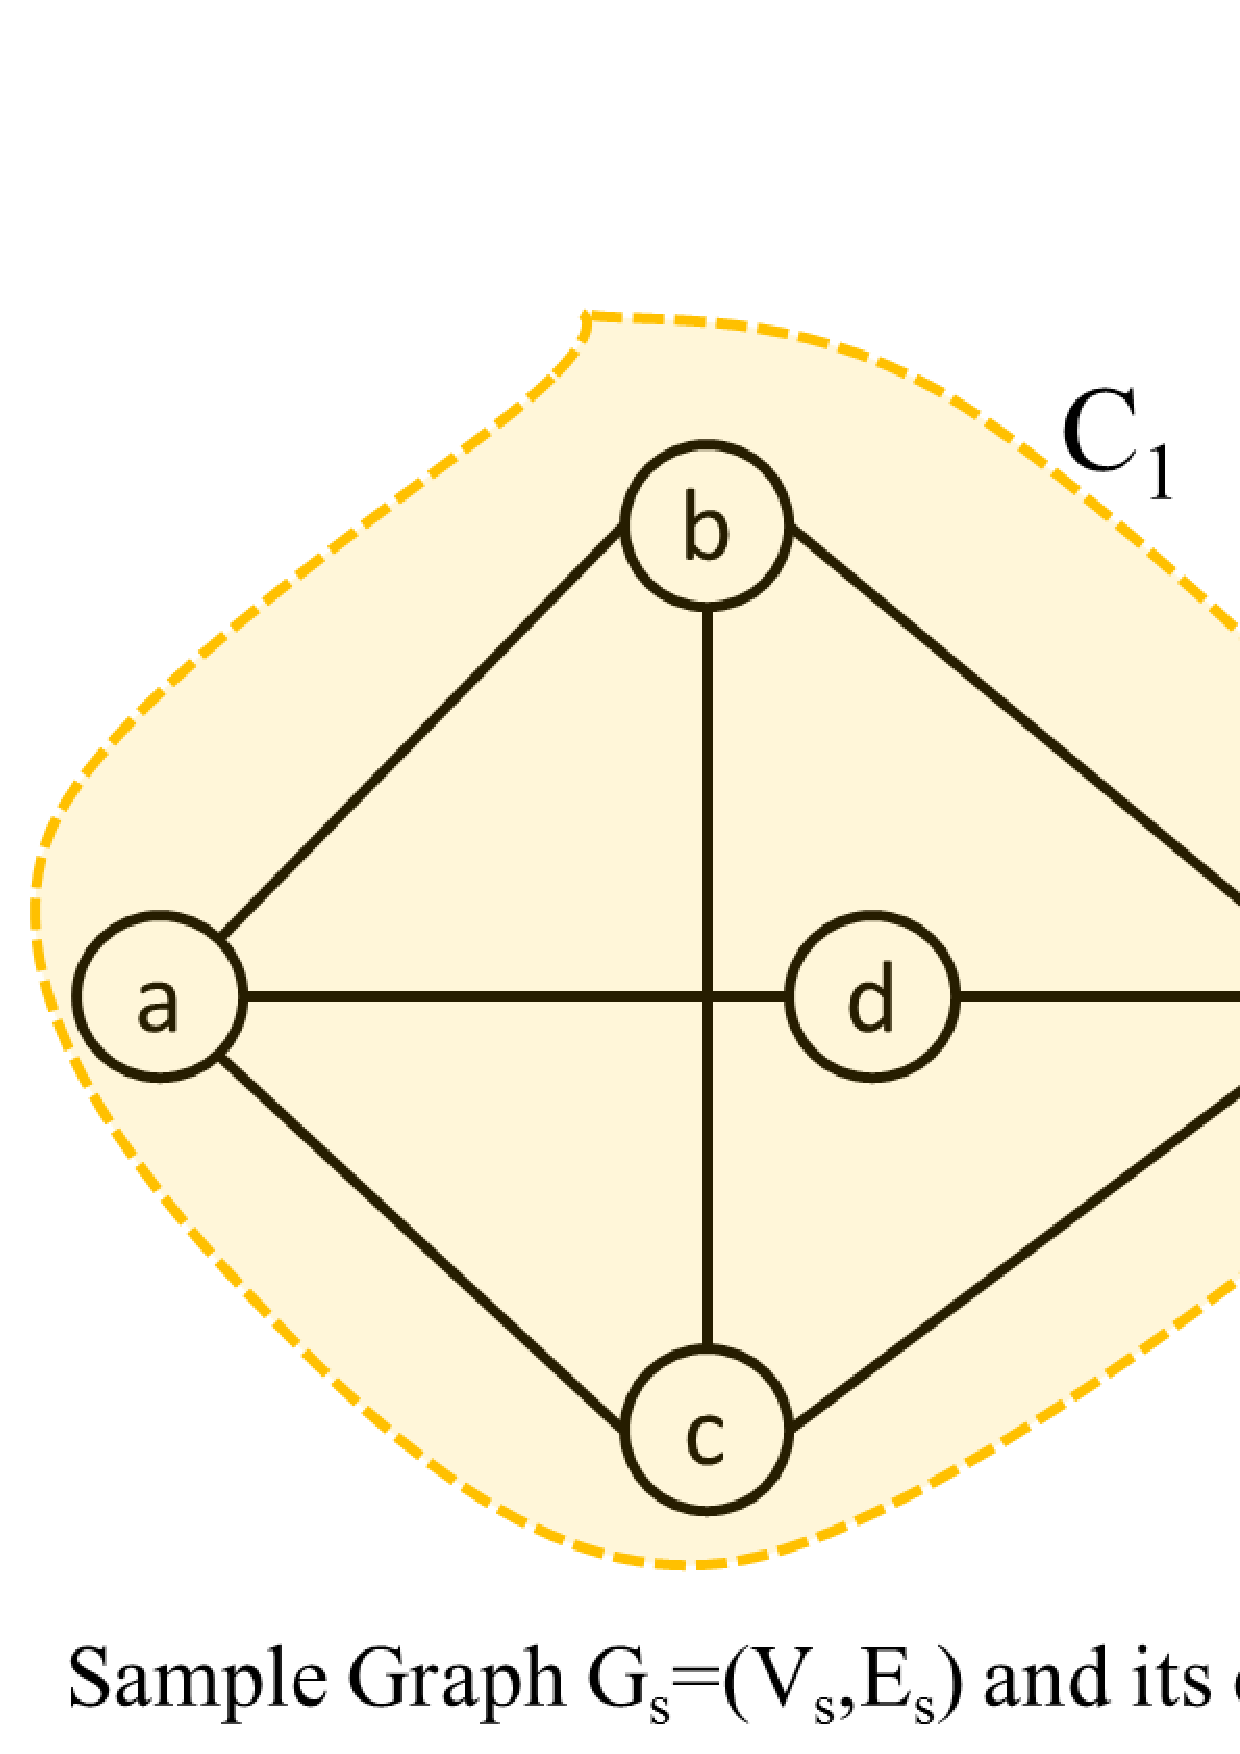
\includegraphics[width=0.8\columnwidth]{./texfiles/Chapter_2/figures/demo.pdf}
%\vspace{-5mm}
\caption{Toy example depicting various conditions handled by \compas~ when a streaming edge arrives.}\label{fig_algo} 
\vspace{2mm}
\end{figure}

%\vspace{-3mm}






\iffalse
\begin{prop}\label{3}
If a new inter-community edge $(u,v)$ connecting two communities $C(u)$ and $C(v)$ is introduced, $C(u)$ $($or $C(v))$ is the most likely candidate for $v$ (or $u$) if it changes its membership.
%\vspace{-2mm}
\end{prop}

\begin{proof}
The method is inspired by \cite{PhysRevE.78.046115} that a vertex $u$ is influenced by two factors: $F^c_{in}(u)$ the force that keeps $u$ stay in its own community $c$, and $F^c_{out}(u)$, the force that a community $S$ imposes to $u$ in order to bring $u$ to $S$ as follows:
\[\small
F^c_{in}(u)=e_c^u-\frac{d_u(D_c-d_u)}{2M}
\]
and 
\[\small
F^S_{out}(u)=max_{S\in NC(u)} \{e_S^u - \frac{d_u D_{outS}}{2M}\}
\]
where $NC(u)$ is the set of neighboring communities of $u$, and $D_{outS}$ is the total degree of vertices outside $S$.

Now we will show that the presence of new edge $(u,v)$ will strengthen $F^{C(v)}_{out}(u)$ and weaken $F^S_{out}(u)$. In other words, we will show that $F^{C(v)}_{out}(u)$ increases while $F^S_{out}(u)$ decreases for all $S \in C \wedge S \notin \{C(u),C(v)\}$.
\[\small
\begin{split}
&F^{C(v)}_{out}(u)|_{new} - F^{C(v)}_{out}(u)|_{old}\\
&=(e_u^{C(v)}+1-\frac{(d_u+1)(d_{outC(v)}+1)}{2(M+1)} - (e_u^{C(v)} - \frac{d_ud_{outC(v)}}{2M})\\
%&= \frac{2M+d_ud_{outC(v)}}{2(M+1)} - \frac{d_ud_{outC(v)}+d_{outD(v)}+d_u+1}{2(M+1)}\\
&\geq \frac{2M+d_ud_{outC(v)}}{2(M+1)} - \frac{d_u d_{outC(v)}+d_{outC(v)}+d_u+1}{2(M+1)}\\
&>0
\end{split}
\]
Therefore $F^{C(v)}_{out}(u)$ is strengthened when a new edge $(u,v)$ is introduced. Further, for any community $S\in C \wedge S\notin \{C(u),C(v)\}$
\[
\begin{split}
& F^{S}_{out}(u)|_{new} - F^{S}_{out}(u)|_{old}\\
&= (e^S_u-\frac{(d_u+1)d_{outS}}{2(M+1)}) - (e^S_u - \frac{d_ud_{outS}}{2M})\\
&= d_{outS}(\frac{d_u}{2M} - \frac{d_u+1}{2(M+1)})<0
\end{split}
\]

This implies that $F^S_{out}(u)$ is weakened when $(u,v)$ is added. Therefore,  the proposition holds.
\end{proof}
\fi


\iffalse
\begin{prop}\label{complex}
If a new edge $(u,v)$ is added into the graph, then joining $u$ to $v$'s  community $C(v)$ will increase the modularity value  if $\Delta Q(u,C(u),C(v)) \equiv 4(M+1)(e_{C(v)}^u+1-e_{C(u)}^u)+e_{C(v)}^u(2D_{C(v)}-2d_u-e_{C(u)}^u) - 2(d_u+1)(d_u+1+d_{C(v)}-d_{C(u)})>0$.
%\vspace{-2mm}
\end{prop}
\fi
\iffalse
\begin{proof}
Vertex $u$ will leave its current community $C(u)$ and join $v$'s community $C(v)$ if
\[\small
\begin{split}
& Q_{C(v)+u} + Q_{C(u)-u} > Q_{c(u)} + Q_{C(v)}\\
&\Leftrightarrow \frac{m_{C(v)}+e_{C(v)}+1}{M+1} - \frac{(d_{C(v)}+d_u+2)^2}{4(M+1)^2}+\\
&\frac{m_{C(u)} - e_{C(u)}}{M+1} - \frac{(d_{C(u)}-d_u-e_{C(u)})}{4(M+1)^2} \\
& > \frac{m_{C(v)}}{M+1} - \frac{(d_{C(v)}+d_u+2)^2}{4(M+1)^2} + \frac{m_{C(u)}}{M+1} - \frac{(d_{C(u)}+1)^2}{4(M+1)^2}\\
&\Leftrightarrow 4(M+1)(e_{C(v)} +1 -e_{C(u)}) + e_{C(u)}(2d_{C(v)} - 2d_{C(u)}-e_{C(u)})\\
& - 2(d_{C(u)}+1)(d_{C(u)}+1+d_{C(v)}-d_{C(u)})>0
\end{split}\]
\end{proof}
\fi
\iffalse
\noindent{\bf Corollary 1.} {\em If the condition in Proposition \ref{complex} is not satisfied, then neither $u$ nor its neighbors should be assigned to $C(v)$.}
\fi

%\vspace{-3mm}

%\vspace{-2mm}
\iffalse
\begin{function2}[!t]\tiny
\caption{\small$OneinSampleOneNew(u,v,e_t,V_s,E_s,\mathcal{H},C_s)$}
\label{onesampleonenew}
\If{$\mathcal{H}$ is not full}{
Insert $v$ to $\mathcal{H}$\\
}
\Else{
Choose a node $x$ with $\mathcal{P}(x) \in V_s$ from $\mathcal{H}$ preferentially based on $\mathcal{H}_c$\\
$V_s,E_s,C_s,\mathcal{H} = OneinSampleOneinBuffer(\mathcal{P}(x),x,V_s,E_s,\mathcal{H},C_s)$\\
%Remove $x$ from $\mathcal{H}$\\
%$\mathcal{H}_c[x]=0$\\
%$\mathcal{H}_p[x]=\phi$\\
%$V_s,E_s,C_s = CheckResizeSample(V_s,C_s,n,1)$\\
%$V_s=V_s\cup x$\\
%$E_s=E_s\cup \{P(x),x\}$\\
%$C_s(x)=C_s(P(x))$\\
%Update $C_s$\\ %\TODO{Not clear what this line does. I do not see a separate update function.}\\
%Insert $v$ to $\mathcal{H}$\\
}

$\mathcal{H}_c[v]=1$\\ 
$\mathcal{H}_p[v]=u$\\ 
\Return $V_s,E_s,C_s,\mathcal{H}$   
\end{function2}
\fi

\begin{function2}[!ht]
\caption{\small $NodeinBuffer(u,\mathcal{H})$}
\label{nodebuffer}
$\mathcal{H}_c[x]=\mathcal{H}_c[x] + 1$\\
\Return $\mathcal{H}$
\end{function2}



%\vspace{-3mm}


\noindent\textbf{(ii) \underline{Both $u$ and $v$ are in buffer:}}
The only action (lines 16 - 18 of Algorithm 1) taken is that in the buffer $\mathcal{H}$, $\mathcal{H}_c$ entries of $u$ and $v$ are incremented by 1 which is achieved through the function $NodeinBuffer()$ (executed twice with $u$ and $v$).
Example: edge $\{k,n\}$ in figure \ref{fig_algo}.

\iffalse
%\vspace{-2mm}
\begin{function3}[!t]\tiny
\caption{\small$BothinBuffer(u,v,\mathcal{H})$}
\label{bothbuffer}
$\mathcal{H}_c[u]=\mathcal{H}_c[u] + 1$\\
$\mathcal{H}_c[v]=\mathcal{H}_c[v] + 1$\\
\Return $\mathcal{H}$
\end{function3}
\fi
%\vspace{-2mm}

%\vspace{-3mm}
\noindent\textbf{(iii) \underline{$u$ is in sample and $v$ is in buffer:}} 
In this case (edge $\{d,i\}$ in Figure \ref{fig_algo}) also the only action (lines 19 - 20 of Algorithm 1) taken is that in the buffer $\mathcal{H}$, $\mathcal{H}_c$ entry of $v$ is incremented by 1 which is implemented through the function $NodeinBuffer()$.

%\noteng{I dont think the next lines are needed}
%In this case (edge $\{d,i\}$ in Figure \ref{fig_algo}), $OneinSampleOneinBuffer()$ (see Function \ref{onesampleonebuffer}) is called from line 19 of Algorithm 1. 
%We first check the sample size constraint (line 4 in Function \ref{onesampleonebuffer}) and accordingly add $v$ (and edge $\{u,v\}$) into $G_s$. $v$ is further assigned to $C(u)$.
\iffalse
%\vspace{-3mm}
\begin{function4}[!h]\tiny
\caption{\small$OneinSampleOneinBuffer(u,v,V_s,E_s,\mathcal{H},C_s)$}
\label{onesampleonebuffer}
%Remove $v$ from $\mathcal{H}$\\
$\mathcal{H}_c[v]=\mathcal{H}_c[v] + 1$\\
$\mathcal{H}_p[v]=u$\\
%$V_s,E_s,C_s = CheckResizeSample(V_s,C_s,n,1)$ \\
%$V_s=V_s\cup v$\\
%$E_s=E_s \cup \{ v,\mathcal{P}(v)\}$\\
%\If{$V_s == n$}{
%Remove one nodes (and all adjacent edges) from $G_s$ having lowest degree \\
%$C_s=CommunityAfterNodeRemove()$;
%}
%$C_s(v)=C_s(u)$\\
%Update $C_s$ \\
%\TODO{Not clear what this line does. I do not see a separate update function.}\\
\Return $V_s,E_s,C_s,\mathcal{H}$   
\end{function4}
\fi
%\vspace{-3mm}

\subsubsection{Entry of a new node:} In the three subsequent cases, at least one node is neither present in the buffer nor in the sample (new). This node triggers a rearrangement, whereby, another selected node is removed from the buffer to make space for the new node, and this selected node is inserted into the graph sample $G_s$  which further triggers a rearrangement of the sample in case it has already reached its size limit ($n$). The function $NodeisNew()$ is invoked to accomplish this task. The rearrangements that take place are described next.

%in order to provide space to the incoming node, a selected node in the buffer replaces a selected node in $G_s$. More specifically three 




%\vspace{-7mm}
\begin{figure}[!h]
\centering
%\vspace{-3mm}
\includegraphics[width=0.8\columnwidth]{./texfiles/Chapter_2/figures/percolation}
\caption{Illustrative example of 3-clique percolation. Once node $g$ is removed, a 3-clique is placed on node $a$. The clique  percolates and accumulates all the nodes except node $f$ which forms a singleton community along with $\{a,b,c,d,e\}$.}\label{fig_percolation} 
%\vspace{-3mm}
\end{figure}


\noindent\underline{Remove node from buffer:} This is triggered when $\mathcal{H}$ is full and in order to make room for the new node one of the existing nodes need to be removed from $\mathcal{H}$. To this aim 
we preferentially remove $x$ from $\mathcal{H}$ based on the counts in $\mathcal{H}_c$ with the 
additional constraint that $\mathcal{P}(x)$ is present in $G_s$. We add node $x$ and edges $\{\mathcal{P}(x)$,$x$\}, into $G_s$. This is achieved by executing the function $RemoveNodefromBuffer()$. 
%Finally, $u$ and $v$ are inserted into $\mathcal{H}$. If during the insertion into $G_s$ the sample size is violated, the required number of nodes along with their adjacent edges are deleted from $G_s$ using $CheckResizeSample()$.

\begin{function3}[!ht]
 \caption{\small $RemoveNodefromBuffer(\mathcal{H},V_s,E_s,C_s)$}
 \label{removenodebuffer}
 Choose $x$ preferentially from $\mathcal{H}$ $\mathcal{P}(x) \in V_s$ \\
 Remove $x$ from $\mathcal{H}$ \\
 $InsertNodeinSample(x,\mathcal{P}(x),V_s,E_s,C_s)$ \\
 \Return  $\mathcal{H},V_s,E_s,C_s$ 
\end{function3}

\noindent\underline{Selection of node for removal from $G_s$:}
Insertion of a node into $V_s$  (obtained in the previous step), 
%we check whether its insertion with exceed the sample size limit. In case it does another rearrangement of $V_s$ is triggered as 
necessitates the removal of an existing node from the sample ($V_s$) to make space for the new entry. 
%Therefore, we first select 
Nodes with the lowest degree in $G_s$ are candidates for deletion. Among these candidate nodes the one (say $x$) with  the lowest clustering coefficient is then removed from the $G_s$ to allow insertion of a new node (selected in the previous step). Subsequently, all the edges incident on $x$ are removed from $G_s$. The function $CheckResizeSample()$ implements this task. Finally, the selected node ($x$) is inserted into $V_s$ utilizing the function $InsertNodeinSample()$, whereby, an edge $(x,\mathcal{P}(x))$ is added to $V_s$ and $x$ is assigned the community of $\mathcal{P}(x)$. 

\begin{function4}[!ht]
\caption{\small$CheckResizeSample(V_s,C_s,n,m)$}
\label{resizesample}
\If{$V_s == n$}{
Remove $m$ nodes say, $u_1, u_2,\cdots, u_m$  (and all their adjacent edges) from $G_s$ having lowest degree and clustering coefficient\\
\For{$u\in \{u_1,u_2,\cdots,u_m\}$}{
$C_s \leftarrow CommunityAfterNodeRemoval(u,C_s)$
}
}
\Return $V_s,E_s,C_s$
\end{function4}

\begin{function5}[!ht]
 \caption{\small $InsertNodeinSample(x,\mathcal{P}(x),V_s,E_s,C_s)$}
 \label{insertnodesample}
 $V_s,E_s,C_s=CheckResizeSample(V_s,E_s,C_s,n,1)$ \\
 $V_s = V_s \cup x$ \\
 $E_s = E_s \cup \{x,\mathcal{P}(x)\}$ \\
 $C_s(x) = C_s(\mathcal{P}(x))$ \\
 Update $C_s$
 \Return $V_s,E_s,C_s$
\end{function5}


\noindent \underline{Adjust communities after removing a node:} 
Deletion of a node might keep the previous community structure unchanged, or break the community into smaller parts, or merge several communities together. The community structure $C_s$ is adjusted using  $CommunityAfterNodeRemoval()$ (Function \ref{communityadjust}) incrementally.  In the extreme,
%Let us consider two extreme cases -- a node with degree $1$ is removed, and a node with highest degree is removed. Removal of a single degree node will keep the community unchanged. However, 
removal of a node might render the community disconnected 
%\noteng{not necessarily}\textcolor{blue}{it has been argued in this paper} 
or broken into smaller parts which might further merge to the other existing communities~\cite{pone.0091431}. Here we utilize the clique percolation method~\cite{PalEtAl05} to handle this situation. In particular, when a vertex $v$ is removed from a community $C$, we place a 3-clique on one of its neighbors and let the clique percolate until no vertices in $C$ are discovered. Nodes discovered in each such clique percolation will form a community. We repeat this clique percolation from each of $v$'s neighbors until each member in $C$ is assigned to a community. For example, in figure \ref{fig_percolation} when node $g$ is removed, we place a 3-clique on its neighbor $a$. Once the 3-clique starts percolating, it accumulates all nodes except $f$. Therefore, two new communities $\{a,b,c,d,e\}$ and $\{f\}$  emerge due to the deletion of $g$. In this way, we let the remaining nodes of $C$ choose their best communities to merge in. % \TODO{It is not clear how you make a community merge into the best possible candidate. In fact, this part is extremely hard to follow. More detailed and explanatory writing + a figure to illustrate the situation is needed {\color{blue} Done}}.
%\vspace{-3mm}
\begin{function6}[!ht]
\caption{\small$CommunityAfterNodeRemoval(u,C_s)$}
\label{communityadjust}
Assume node $u$ and its adjacent edges are removed from $G_s$\\
$i=1$\\
\While{$N(u)\neq \phi$}{
$b_i$=Nodes found by a 3-clique percolation on $v\in N(u)$\\
\If{$b_i==\phi$}{
$b_i=\{v\}$
}
$C_s=C_s \cup b_i$\\
$N(u)=N(u)\setminus b_i$\\
$i=i+1$\\
}
%Let each singleton in $N(a)$ consider its best communities \TODO{Not clear how this is done?}\\
%Let each $b_i$ consider its best communities \TODO{Not clear how this is done?}\\
Update $C_i$\\% \TODO{What does this line do?}\\
\Return $C_s$   
\end{function6}


We now proceed to discuss the remaining cases. \\
\noindent\textbf{(iv) \underline{$u$ is in sample and $v$ is new:}}
In this case (handled by lines 21 - 22 in Algorithm 1) $v$ is inserted into the buffer $\mathcal{H}$ if $\mathcal{H}$ is not full. Otherwise its insertion triggers rearrangements of $\mathcal{H}$ and subsequently $V_s$. We use $NodeisNew()$ to accomplish this task. 

% \noteng{I think in general put examples at the end}
% When a new node $v$  connecting node $u\in G_s$ appears, $OneinSampleOneNew()$ (see Function \ref{onesampleonenew}) is executed 
% (line 17 of Algorithm 1, edge $\{b,p\}$ in Figure \ref{fig_algo}). In this case, we do not add $\{u,v\}$ into the sample immediately. Instead, we first 
% insert $v$ into $\mathcal{H}$ if $\mathcal{H}$ is not full. If $\mathcal{H}$ is full, we preferentially pick a node $x$ based on $\mathcal{H}_c[x]$ with $\mathcal{P}(x) \in G_s$ and then execute $OneinSampleOneinBuffer()$ (Function \ref{onesampleonebuffer}, discussed later) with $\mathcal{P}(x)$ and $x$.  
%\textcolor{green}{
%The idea is to delay the insertion of the node into the sample in order to estimate its importance (current hit count) prior to insertion. This further ensures the insertion of high degree nodes in the sample.
%}
% If $\mathcal{H}$ is full, we pick one node $x$ from $\mathcal{H}$ preferentially based on $\mathcal{H}_c[x]$ with an additional constraint that $\mathcal{P}(x)$, 
% the parent of $x$  should be in $G_s$\footnote{\textcolor{green} {this additional constraint allows to avoid a disconnected component being created in the sample and at the same time expanding the giant component.}} (e.g., 
% in Figure~\ref{fig_algo} if the buffer is full although node $l$ has highest count we do not pick $l$ from the buffer because its parent node $i$ is not in $G_s$; 
% instead we pick $m$ which satisfies both the constraints). $x$ is then added to $G_s$ through the edge $\{\mathcal{P}(x),x\}$ (line 10 in Function 2) and is assigned 
% the community of $\mathcal{P}(x)$ (line 11 in Function 2). 
%We also check if including $x$ in $G_s$ violates the sample size constraint through the function 
%If $G_s$ is already full (i.e., $V_s=n$) then 
%$CheckResizeSample()$ (Function 7). 
% If $G_s$ is already full (i.e., $V_s=n$), one existing node which has lowest degree is removed from $G_s$ and the community structure 
% is adjusted accordingly using $CommunityAfterNodeRemoval()$ (both Functions 7 and 8 are discussed later).

%If $\mathcal{H}$ is full, we will remove one node $x$ from $\mathcal{H}$ preferentially based on the  number of times $x$ is encountered previously and add it into $G_s$. To do so, we first check if $P(x)$, the parent of $x$ is already in $G_s$; if exists then we assign $x$ into the community of $P(x)$ (line 11 of Function 2). We also check if assigning $x$ into $G_s$ will not violate the size of $G_s$. If $G_s$ is already full (i.e., $V_s$=n) then we call $CheckResizeSample()$ (Function 6) which will remove  from $G_s$ one existing node which has lowest degree and adjust the community accordingly using $CommunityAfterNodeRemoval()$ (discussed later in Function 7). On the other hand, if $P(x)$ is not in $G_s$ but in $\mathcal{H}$, we remove both $x$ and $P(x)$ from $\mathcal{H}$ and add them into $G_s$. Once again, if $G_s$ is full, two nodes are removed from $G_s$ based on the lowest degree as mentioned earlier and communities are adjusted (line 18 in Function 2). Then a new community is created, and $x$ and $P(x)$ are added into it (line 22 in Function 2).





%\vspace{-3mm}
 
%\vspace{-1mm}
\noindent\textbf{(v) \underline{$u$ is in buffer and $v$ is new:}} In this case (edge $\{m,p\}$ in Figure \ref{fig_algo}), we increment the counter corresponding to $u$ and attempt to insert $v$ into $\mathcal{H}$ using the function $NodeisNew()$. 

\begin{function7}[!ht]
 \caption{\small $NodeisNew(u,v,\mathcal{H},V_s,E_s,C_s)$}
 \label{nodenew}
 \If{$\mathcal{H}$ is full}{
$RemoveNodefromBuffer(\mathcal{H},V_s,E_s,C_s)$ \\
}
Insert u in $\mathcal{H}$ \\
$\mathcal{H}_c[u] = 1$\\
$\mathcal{H}_p[u] = v$ \\

\Return $\mathcal{H},V_s,E_s,C_s$
\end{function7}

%see Function \ref{onebufferonenew}) is similar to Function 2. We first increment the counter corresponding to $u$ in the buffer and add $v$ into the buffer in the same way as mentioned in Function 2.\noteng{What is function 2 does it cover the entire three-step process}
%\vspace{-4mm}
\iffalse
\begin{function7}[!h]\tiny
\caption{\small$OneinBufferOneNew(u,v,e_t,V_s,E_s,\mathcal{H},C_s)$}
\label{onebufferonenew}
$\mathcal{H}_c[u]=\mathcal{H}_c[u]+1$\\
$V_s,E_s,C_s,\mathcal{H} = OneinSampleOneNew(u,v,e_t,V_s,E_s,\mathcal{H},C_s)$\\
\Return $V_s,E_s,C_s,\mathcal{H}$  %\TODO{Check. I think we do not need this line as it is included already in the previous function.{\color{blue}Done}}
\end{function7}
%\vspace{-4mm}
\fi

\noindent\textbf{(vi) \underline{Both $u$ and $v$ are new:}}
In this case we attempt to insert both $u$ and $v$ to the buffer by executing the function $NodeisNew()$. 

Summarizing, the algorithm continuously increases the proportion of high fidelity nodes and 
improves the community structure by the following actions -- 
%We would like to point out that although our algorithm follows a greedy approach, it is able to achieve its objective of obtaining a sample that preserves the underlying community structure. In specific - \\
(a) delaying the insertion of a node to the sample allows for determining the importance of a node.\\
(b) removal of low clustering coefficient nodes from the sample ensures that only nodes with high clustering coefficient constitute the final $G_s$.  \\
(c) since all the actions are aimed at improving  modularity at every iteration, the final $G_s$ potentially will have 
 well-separated community structure.   

%\noteng{This would also trigger Function2}
%When both $u$ and $v$ are new (edge $\{p,q\}$ in Figure \ref{fig_algo}), $BothNew()$ (see Function \ref{bothnew}) is called from line 23 of Algorithm 1. %We initially check whether buffer $\mathcal{H}$ is full or not. In case it is not full, we insert $u$ in $\mathcal{H}$ and then call Function 2. Otherwise, 
%{\em Selection of nodes from buffer:} We preferentially remove $x$ and $y$ from $\mathcal{H}$ based on the counts in $\mathcal{H}_c$ with the additional constraint that both $\mathcal{P}(x)$ and $\mathcal{P}(y)$ are in $G_s$, and add nodes $x$, $y$ and edges $\{\mathcal{P}(x)$,$x$\}, $\{\mathcal{P}(y)$,$y\}$ into $G_s$. $x$ and $y$ are also assigned to the community of the their respective parents. Finally, $u$ and $v$ are inserted into $\mathcal{H}$. If during the insertion into $G_s$ the sample size is violated, the required number of nodes along with their adjacent edges are deleted from $G_s$ using $CheckResizeSample()$.

\iffalse
%\vspace{-3mm}
\begin{function8}[!t]\tiny
\caption{\small$BothNew(u,v,e_t,V_s,E_s,\mathcal{H},C_s)$}
\label{bothnew}
\If{$\mathcal{H}$ is not full}{
Insert $u$ to $\mathcal{H}$\\
$\mathcal{H}_p[u] = v$\\
$\mathcal{H}_c[u] = 1$\\
$V_s,E_s,C_s,\mathcal{H}= OneinSampleOneNew(u,v,e_t,V_s,E_s,\mathcal{H},C_s)$\\
}
\Else{
Choose nodes $x$, $y$ with $\mathcal{P}(x), \mathcal{P}(y) \in V_s$\TODO{Not $\mathcal{P}(y) \in V_s$?}\textcolor{blue}{corrected} from $\mathcal{H}$ preferentially based on $\mathcal{H}_c$\\
Remove $x$, $y$ from $\mathcal{H}$\\
$\mathcal{H}_c[x] = 0$, $\mathcal{H}_c[y] = 0$\\
$\mathcal{H}_p[x] = \phi$, $\mathcal{H}_p[y] = \phi$\\
$V_s,E_s,C_s = CheckResizeSample(V_s,C_s,n,2)$\\
$V_s = V_s \cup x \cup y$ \\
$E_s = E_s \cup \{x,\mathcal{P}(x)\} \cup \{y,\mathcal{P}(y)\}$ \\
$C_s(x) = C_s(\mathcal{P}(x))$\\
$C_s(y) = C_s(\mathcal{P}(y))$\\
Update $C_s$\\ % \TODO{Not clear how this function helps?}\\
Insert $u,v$ to $\mathcal{H}$\\
$\mathcal{H}_p[u] = v$, $\mathcal{H}_p[v] = u$ \\
$\mathcal{H}_c[u] = 1$, $\mathcal{H}_c[v] = 1$\\

}
\Return $V_s,E_s,C_s,\mathcal{H}$   %\TODO{Check: the if part does not need this return as the function preceding already does it. Only the second part needs it? {\color{blue} Done}}
\end{function8}
\fi
%\vspace{-3mm}

\iffalse
\begin{figure}[!t]
\centering
%\vspace{-3mm}
\includegraphics[width=\columnwidth]{figures/percolation}
\caption{Illustrative example of 3-clique percolation. Once node $g$ is removed, a 3-clique is placed on node $a$. The clique  percolates and accumulates all the nodes except node $f$ which forms a singleton community along with $\{a,b,c,d,e\}$.}\label{fig_percolation} 
%\vspace{-3mm}
\end{figure}
\fi
%\noteng{The algorithm has huge complexity}


%{\color{red}
%1. When blindly enter the edges, do we increase the counter.\\
%2. Assume that $G_s$ can take only one node. If you try to add $u,v$ together, what would happen\\
%3. No edge deletion case in your algorithm\\
%4. In case of BothNew, if buffer has only one vacant place, what would happen. For me, we should add $u$ and $v$ one by one and follow the previous step, instead of adding together,
%}



%\vspace{-3mm}

\section{Experimental Setup}
%In this section we evaluate the effectiveness of our algorithm as compared to the existing methods. We start by explaining the datasets and baseline sampling algorithms. Then we provide the criteria to evaluate the competing algorithms, followed by a detailed comparative analysis. 
In this section, we describe the baseline sampling algorithms and the datasets used in our experiments.

\subsection{Sampling algorithms}
We compare \compas~ with five existing sampling methods: (i) Streaming Node (SN) \cite{ahmed2014network}, (ii) Streaming Edge (SE) \cite{ahmed2014network}, (iii) Streaming BFS (SBFS) \cite{ahmed2014network}, (iv) PIES \cite{ahmed2014network}, and (v) Green algorithm (GA) \cite{tong2016novel}. The first four algorithms are exclusively designed for streaming graphs while the last one is designed for static graphs. Note that unlike ours, none of the existing methods explicitly produce a community structure as a by-product of the sampling,
%\footnote{Although GA claims that its sample graph preserves the underlying community structure, it does not explicitly produce the community structure.}, 
and thus one needs to execute community detection algorithm separately on the sample to obtain the community structure. Therefore to evaluate the competing methods w.r.t how the underlying community structure in the sample resembles with that of the original graph, for SN, SE, SBFS and PIES we run Louvain algorithm~\cite{blondel2008fast}
\footnote{We also considered other algorithms (CNM \cite{clauset2004finding}, GN \cite{girvan2002community} and Infomap \cite{rosvall2008maps}) and found the results to be similar.} 
%\noteng{are there results on that?} \textcolor{blue}{Yes}
%} 
on each individual sample and detect the communities. In case of GA, we consider the aggregated graph and run GA to obtain the sample, and further run Louvain algorithm on the sample to detect the community structure. 
Note that although by considering the aggregated graph, GA acquires far more information of the entire graph structure, we use it as a strict baseline in this study.
%to show that the community structure obtained from \compas~is quite competitive to that obtained by running community detection on GA's sample graph.   

\begin{table}[]
\centering
\caption{Datasets used for evaluation.}
\label{tab:data}
%\begin{adjustbox}{max width=0.5\textwidth}
\begin{tabular}{l l l l l l}
\hline
Dataset  & Facebook & arxiv hep-th & Youtube   & Dblp      & LFR     \\ \hline
\# Nodes & 63,731   & 22,908       & 1,134,890 & 317,080   & 25,000  \\ 
\# Edges & 817,035  & 2,444,798    & 2,987,624 & 1,049,866 & 254,402 \\ \hline
\end{tabular}
%\end{adjustbox}
%\vspace{2mm}
\vspace{3mm}
\end{table}



%\vspace{3mm}
\subsection{Datasets}\label{sec:dataset}

We perform our experiments on following five graphs  (first two are streaming graphs, and last three are static graphs):  

(i) {\bf Facebook}~\cite{d1}: 
%\footnote{konect.uni-koblenz.de/networks/facebook-wosn-links}: 
An undirected graph where nodes (63,731) are users, and edges (817,035) are friendship links that are time-stamped;  % \TODO{Is there a ground truth community structure? Else how do you obtain communities here?} \textcolor{blue}{done}\\

(ii) {\bf arxiv hep-th}\footnote{konect.uni-koblenz.de/networks/ca-cit-HepTh}: 
Here nodes (22,908) are authors of arXiv's High Energy Physics papers and an edge exists between two authors if they have co-authored a paper; edges (2,444,798) are time-stamped by the publication date;% \TODO{Is there a ground truth community structure? Else how do you obtain communities here?}\textcolor{blue}{done}\\ 
 
 (iii) {\bf Youtube}\footnote{snap.stanford.edu/data/com-Youtube.html}:
Nodes (1,134,890) represent Youtube users and edges (2,987,624) representing friendship.
%User created groups in the network form the ground truth community structure. There are 8,385 communities in the ground truth.\\

(iv) {\bf dblp}\footnote{snap.stanford.edu/data/com-DBLP.html}:
This dataset consists of authors indexed in DBLP. The graph is same as arxiv hep-th (317,080 nodes and 1,049,866 edges).

(v) {\bf LFR}~\cite{lancichinetti2008benchmark}: This is a synthetic graph with underlying community structure implanted into it (Table \ref{tab:data}).
We construct the graph with 25,000 nodes, 254,402 edges and 1,834 communities.
%{\color{red} put \# of nodes and edges}
%The first three datasets were presented by Yang et.~al. in \cite{yang2015defining}.
%Although the above graphs are all static, we assign 

Since last three graphs are static, we consider that each edge arrives in a pre-decided (random) order, i.e., each edge has a (discrete) time of arrival. 
The edge ordering, as we shall see, does not influence the inferences drawn from the results.
Moreover, since first four graphs do not have any underlying ground-truth community structure, we run Louvain algorithm %\cite{blondel2008fast} {\color{red} only louvain?} 
on the aggregated graph and obtain the disjoint community structure. This community structure is the best possible output that we can expect from our incremental modularity maximization method, and therefore serves as the ground-truth. 


\begin{table}
\centering
\caption{Summary of the D-statistics (the lower, the better) values of the topological measures for Facebook. Top two values for each average result is highlighted.}
\label{tab_fb}
\begin{adjustbox}{max width=\textwidth}
\begin{tabular}{c|c c c c c c c c c c c c c |c}
\hline
Algorithm & ID & EI & AD & FOMD & TPR & EX & CR & CON & NC & AODF & MODF & FODF & MOD & Avg \\ \hline
Compas    & 0.08   & 0.11   & 0.15   & 0.32     & 0.28    & 0.14   & 0.12   & 0.16    & 0.09   & 0.14     & 0.11     & 0.41     & 0.16 & {\bf 0.17}   \\ 
SN        & 0.26         &  0.21   & 0.22   & 0.42     & 0.86    & 0.20   & 0.34   & 0.19    & 0.15   &  0.36    & 0.24     & 0.40     & 0.33 & 0.33    \\ 
SE        & 0.19         &  0.15   & 0.21   & 0.28     & 0.57    & 0.27   & 0.24   & 0.20    & 0.17   & 0.41     & 0.25     & 0.37     & 0.25 & 0.27   \\ 
SBFS      &  0.25        &  0.29   & 0.27   & 0.38     & 0.28    & 0.18   & 0.15   & 0.17    & 0.16   & 0.26     & 0.27     & 0.48     &  0.26 & 0.26   \\ 
PIES      & 0.27         &  0.28  & 0.30   & 0.31     & 0.41    & 0.17   &  0.23  &  0.21   &  0.30  & 0.35     & 0.37     &  0.29    & 0.28 & 0.29   \\ 
GA        & 0.14   &  0.17   &  0.21   & 0.12     &  0.09   &  0.06  & 0.09   &  0.13    & 0.15   & 0.11     &  0.07      & 0.10   & 0.12 & {\bf 0.12} \\ \hline
\end{tabular}
\end{adjustbox}
\vspace{3mm}
\end{table}


%\vspace{-3mm}
\section{Evaluation}
\iffalse
We design a two-fold experimental setup. First, we show how  competing sampling algorithms detect the original community structure, and second, we measure how good individual samples are w.r.t. the structural properties of the original graph. Although the primary focus of \compas~is to improve upon in the first evaluation, we also show that it is quite competitive in terms of the second evaluation.
\fi

\begin{table}
\centering
\caption{Summary of the D-statistics values of the topological measures for arxiv hep-th graph.}
\label{tab_hep-th}
\begin{adjustbox}{max width=\textwidth}
\begin{tabular}{c|c c c c c c c c c c c c c | c}
\hline
Algorithm & ID & EI & AD & FOMD & TPR & EX & CR & CON & NC & AODF & MODF & FODF & MOD & Avg\\ \hline
Compas    & 0.12 & 0.06 &0.09 & 0.06  &  0.14 & 0.13  &  0.10   & 0.09   & 0.07     &   0.16   &  0.06& 0.08   &  0.10 & {\bf 0.10}  \\ 
SN        & 0.29   & 0.25   & 0.28   &  0.22    &  0.19   & 0.32   &  0.24  &  0.20   & 0.21   & 0.28     & 0.33     &   0.26   &  0.31 & 0.26 \\ 
SE        & 0.22   &  0.27  &  0.37  &  0.36    &  0.31   &  0.35  &  0.21  &  0.29   &  0.32  &  0.29    &  0.26    & 0.21     &  0.31 & 0.29  \\ 
SBFS      &  0.22  & 0.27   &  0.26  &  0.18    &   0.38  &  0.31  & 0.34    &  0.21   & 0.25   &  0.23    & 0.25     &  0.26    &  0.22 & 0.26  \\ 
PIES      & 0.15   &  0.21  &  0.23  &  0.27    &  0.14   & 0.24    & 0.26   & 0.23    &  0.17  & 0.21     &  0.13   &  0.19    &  0.29  & 0.21 \\ 
GA        &  0.11  & 0.08   & 0.12   &   0.10   & 0.08    & 0.05   & 0.06   & 0.09    &   0.06 &  0.07    &  0.04    &  0.14 &  0.06 & {\bf 0.08}\\ \hline
\end{tabular}
\end{adjustbox}
\vspace{3mm}
\end{table}


\begin{table}[!t]
\centering
\caption{\label{tab_yt}Summary of the $D$-statistics (the lower, the better) values of the topological measures for Youtube dataset.}
% \TODO{Provide standard deviation/error $\sigma$ for the last 4 networks.}}


\begin{adjustbox}{max width=\textwidth}
\begin{tabular}{c|c c c c c c c c c c c c c | c}
\hline
Algorithm & ID & EI & AD & FOMD & TPR & EX & CR & CON & NC & AODF & MODF & FODF & MOD & Avg \\ \hline
\compas     & 0.06   & 0.05   & 0.08    & 0.06     & 0.23    & 0.08   & 0.05   & 0.09    & 0.26   & 0.07    & 0.20     &  0.12    & 0.05 & {\bf 0.10} \\ 
SN         & 0.16   &  0.17 & 0.47   & 0.06     & 0.54    & 0.58   & 0.11   & 0.26    & 0.06   & 0.16     & 0.18     & 0.09     &  0.22 & 0.23 \\ 
SE         &  0.26  & 0.24   & 0.24   & 0.50     & 0.28    & 0.10   & 0.29   & 0.09    & 0.15  & 0.10     &  0.25    &  0.09    & 0.20  & 0.21 \\ 
SBFS       &  0.13  & 0.13   & 0.17   &  0.10    & 0.45    & 0.14   & 0.06   & 0.16    & 0.04   &   0.26   & 0.11     & 0.08     & 0.18 & 0.15  \\ 
PIES       &  0.23  & 0.24   &  0.25  & 0.19    & 0.41    & 0.04   & 0.05   & 0.05    & 0.06   &      0.16 & 0.04    & 0.05     & 0.12  & 0.14 \\ 
GA         &   0.15 & 0.05   & 0.06   & 0.05     & 0.27    & 0.07   & 0.08   & 0.05    & 0.08   &   0.15   & 0.07     &  0.07    & 0.10 & {\bf 0.09}  \\ \hline
\end{tabular}
\end{adjustbox}
\vspace{3mm}
\end{table}



%\subsection{Community-centric evaluation}
In this section, we list the standard metrics used to evaluate the goodness of the community structure, followed by a detailed comparison of the sampling algorithms.

 {\bf Evaluation criteria:}
To measure how sampling algorithms capture the underlying community structure, we evaluate them in two ways.  First we measure the quality of the obtained community structure based on the {\bf topological measures} defined by \cite{yang2015defining}. In particular, we look into four classes of quality scores - (i) {\em based on internal connectivity}: internal density (ID), edge inside (EI), average degree (AD), fraction over mean degree (FOMD), triangle participation ratio (TPR); (ii) {\em based on external connectivity}: expansion (EX), cut ratio (CR); (iii) {\em combination of internal and external connectivity}: conductance (CON), normalized cut (NC), maximum out-degree fraction (MODF), average out-degree fraction (AODF), flake out-degree fraction (FODF); and (iv) {\em based on graph model}: modularity (MOD).
%\footnote{See~\cite{yang2015defining} for the detailed definitions of all these metrics.}. 
Note, for every individual community we obtain a score, and therefore a distribution of scores (i.e., distribution of ID, EI etc.) is obtained for all the communities of a graph. We measure how similar (in terms of Kolgomorov-Smirnov $D$-statistics\footnote{It is defined as $D = max_x\{|f(x) - f^{'}(x)|\}$ where $x$ is over the range of the random variable, and $f$ and $f^{'}$ are the two empirical cumulative distribution functions of the data.}) these distributions are with those of the ground-truth communities. {\em The less the value of D-statistics, the better the match between two distributions}.

\begin{table}
\centering
\caption{Summary of the D-statistics values of the topological measures for Com-dblp dataset.}
\label{tab_dblp}
\begin{adjustbox}{max width=\textwidth}
\begin{tabular}{c|c c c c c c c c c c c c c | c}
\hline
Algorithm & ID & EI & AD & FOMD & TPR & EX & CR & CON & NC & AODF & MODF & FODF & MOD & Avg\\ \hline
Compas    & 0.13   & 0.07   & 0.13   & 0.10     & 0.12    & 0.12   & 0.11   & 0.13    & 0.11   & 0.37     & 0.05     & 0.41     & 0.16 & {\bf 0.16}  \\ 
SN        &  0.51  & 0.60   & 0.54   & 0.11    & 0.51    & 0.12   & 0.11   & 0.37    & 0.05   & 0.11     &   0.24   & 0.11     & 0.51  & 0.29  \\ 
SE        &  0.51  & 0.49   & 0.48   & 0.27    & 0.24    & 0.12   & 0.13   & 0.12    & 0.11   & 0.21     & 0.12     &  0.18    & 0.23  & 0.25  \\ 
SBFS      &  0.34  & 0.32   & 0.41   & 0.18     & 0.40    & 0.15   & 0.13   &  0.14   & 0.18   &  0.12    &   0.34   & 0.24     & 0.11 & 0.24   \\ 
PIES      & 0.27   &  0.14  & 0.24   &  0.29    & 0.17    & 0.34   & 0.28   &  0.19   &  0.20  & 0.31     & 0.32     &  0.21    &  0.16 & 0.22  \\ 
GA        & 0.13   & 0.16   & 0.11   &  0.05    &  0.17  & 0.08   &  0.15  &  0.14   & 0.19   & 0.07     &  0.10    &  0.09    & 0.12   & {\bf 0.12} \\ \hline
\end{tabular}
\end{adjustbox}
\vspace{3mm}
\end{table}


%We further measure the community quality based on the ground-truth community structure. Finally, we calculate the Kolgomorov-Smirnov $D$-statistics between the community score distribution obtained from the sample and the ground truth for each individual type of score. Note that $D$-statistics is applied as a part of Komogorov-Smirnov test to reject the null hypothesis. Here we use it to measure the agreement between the two distributions. 

As a second level of evaluation, we use the {\bf community validation metrics} --  Purity~\cite{manning2008introduction}, Normalized Mutual Information (NMI)~\cite{danon2005comparing} and Adjusted Rand Index (ARI)~\cite{hubert1985comparing} to measure the similarity between the ground-truth and the obtained community structures. {\em The more the value of these metrics, the higher the similarity.}
\iffalse
\begin{table*}[!t]
\centering
\caption{\label{g_metric_alg}Purity (PU), NMI and ARI values between the ground-truth and community structure obtained from individual sampling algorithms for all datasets.}
\scalebox{0.7}{
\begin{tabular}{l |>{\columncolor[gray]{0.8}} c>{\columncolor[gray]{0.8}}  c>{\columncolor[gray]{0.8}}  c|  c  c  c| ccc|ccc|ccc|>{\columncolor[gray]{0.8}}c>{\columncolor[gray]{0.8}}c>{\columncolor[gray]{0.8}}c}
\hline
\multirow{2}{*}{{\bf Dataset}} & \multicolumn{3}{c|}{{\bf \compas}} & \multicolumn{3}{c|}{{\bf SN}} & \multicolumn{3}{c|}{{\bf SE}} & \multicolumn{3}{c|}{{\bf SBFS}} & \multicolumn{3}{c|}{{\bf PIES}} & \multicolumn{3}{c}{{\bf GA}} \\\cline{2-19}
   & \multicolumn{1}{c}{PU} & \multicolumn{1}{c}{NMI} & \multicolumn{1}{c|}{ARI} & PU & NMI & ARI &PU & NMI & ARI &PU & NMI & ARI &PU & NMI & ARI & \multicolumn{1}{c}{PU} & \multicolumn{1}{c}{NMI} & \multicolumn{1}{c}{ARI} \\\hline
Facebook	  & 0.71 & 0.52 & 0.47	 & 0.43&0.34&0.26  & 0.39&0.28&0.12  &  0.53&0.41&0.18  & 0.57&0.48&0.36  & 0.76&0.61&0.52 \\
hep-th		  &	0.69&0.51&0.38 & 0.39&0.32&0.19 & 0.29&0.21&0.12 & 0.42&0.36&0.25  & 0.48&0.39&0.31 & 0.74&0.68&0.57\\
youtube		      & 0.83&0.72&0.67	 &  0.52&0.49&0.36 & 0.48&0.33&0.28  &  0.63&0.58&0.47 & 0.56&0.51&0.41  & 0.86&0.77&0.71 \\
Dblp		  &	0.72&0.65&0.58 & 0.32&0.28&0.21  & 0.29&0.21&0.16  & 0.66&0.57&0.32  & 0.48&0.39&0.31  & 0.79&0.69&0.52 \\
LFR		  & 0.76&0.69&0.55	 & 0.35&0.29&0.21  & 0.56&0.32&0.29  & 0.49&0.38&0.26  & 0.42&0.31&0.28  &  0.81&0.72&0.67 \\\hline
Average & 0.74 & 0.61 & 0.53 & 0.40 & 0.34 & 0.24 & 0.40 & 0.27 &0.19 & 0.54 & 0.46 & 0.29 & 0.50 & 0.41 & 0.33 & 0.79 & 0.69 & 0.59   \\
\hline
\end{tabular}}
%\vspace{-5mm}
\end{table*}
\fi
%\vspace{-3mm}

\begin{table}
\centering
\caption{Summary of the D-statistics values of the topological measures for LFR graph.}
\label{tab_lfr}
\begin{adjustbox}{max width=\textwidth}
\begin{tabular}{c|c c c c c c c c c c c c c | c}
\hline
Algorithm & ID & EI & AD & FOMD & TPR & EX & CR & CON & NC & AODF & MODF & FODF & MOD & Avg\\ \hline
Compas    &  0.16  &  0.23  &  0.18  &  0.12    &  0.08   & 0.20   &  0.24  &  0.13   & 0.21   &  0.28    &  0.27    &   0.15   & 0.09 & {\bf 0.18}   \\ 
SN        &  0.21  &  0.26  &  0.17  &  0.29    &  0.14   & 0.37   & 0.27   & 0.33    &  0.28  &  0.32    & 0.25     & 0.40     &  0.22 & 0.27  \\ 
SE        & 0.32   & 0.36   &  0.41  &   0.46   &   0.23  & 0.31   & 0.45   &  0.28   & 0.19   &   0.38   &  0.18    &  0.26    & 0.33  & 0.32  \\ 
SBFS      &  0.32  &  0.15  &  0.20  &  0.12    &  0.35   & 0.37   & 0.26   &  0.29   & 0.37   &   0.09   & 0.25     &  0.30    & 0.18  & 0.25  \\ 
PIES      & 0.38   & 0.18   &  0.19  &  0.32    &  0.23   &  0.26  & 0.28   &  0.21   & 0.25   & 0.20     & 0.34     &  0.24    &  0.24 & 0.26  \\ 
GA        &  0.18  &  0.27  & 0.11   & 0.12     &  0.07   & 0.12   &  0.05  &  0.06   & 0.14   &  0.08    &  0.21    &  0.17    & 0.14  & {\bf 0.14}  \\ \hline
\end{tabular}
\end{adjustbox}
\vspace{3mm}
\end{table}

{\bf Parameter estimation}:
As reported in Section~\ref{algorithm},~\compas~ consists of two parameters: (i) $\alpha$ (initial fraction of the nodes inserted), (ii) $n_d$ (length of the buffer).
%In Figures \ref{param_est}(a) and \ref{param_est}(b) we plot the average  $D$-statistics for different values of $\alpha$ and $n_d$ respectively. 
We observe that $D$-statistics is initially high and reduces as we increase $\alpha$ (figures \ref{param_est}(a)). This is because for low $\alpha$, the community structure obtained initially by running a community-detection algorithm (Step 12 in Algorithm 1) is coarse. For large values of $\alpha$ even though initial community structure obtained is good, it is not allowed to evolve much. Similarly, in figure~\ref{param_est}(b), given a small buffer size several nodes mostly arriving once would be added to the sample leading to formation of pendant vertices. As we increase the buffer size \compas~performs better till a certain point, after which the improvement is negligible. Since we are interested in using minimum space we fix $n_d$ at $0.0075 n$. Similarly $\alpha$ is set to $0.4$. 
%Thus, for the rest of the experiments we set $\alpha$ to $0.5$ and $n_d$ to $0.0075n$ unless otherwise specified. 
We also set $n$ to $0.4|V|$ as default (see Section \ref{sec:effect} for different values of $n$). Further note that apart from Louvain we also consider other algorithms (CNM~\cite{clauset2004finding}, GN~\cite{girvan2002community} and Infomap~\cite{rosvall2008maps}) for obtaining the initial community structure. 
%{\color{red} may be Infomap, then remove "modularity optimization"}. 
The average $D$-statistics values (calculated for LFR) across all the quality scores for Louvain, CNM, GN and Infomap are respectively \textbf{0.182}, \textbf{0.191}, \textbf{0.216} and \textbf{0.197}. 
Above results indicate that \compas~ is independent of the community detection algorithm used initially and we thus stick to Louvain for evaluation.

%\vspace{-2mm}
\begin{figure}[!h]
\centering
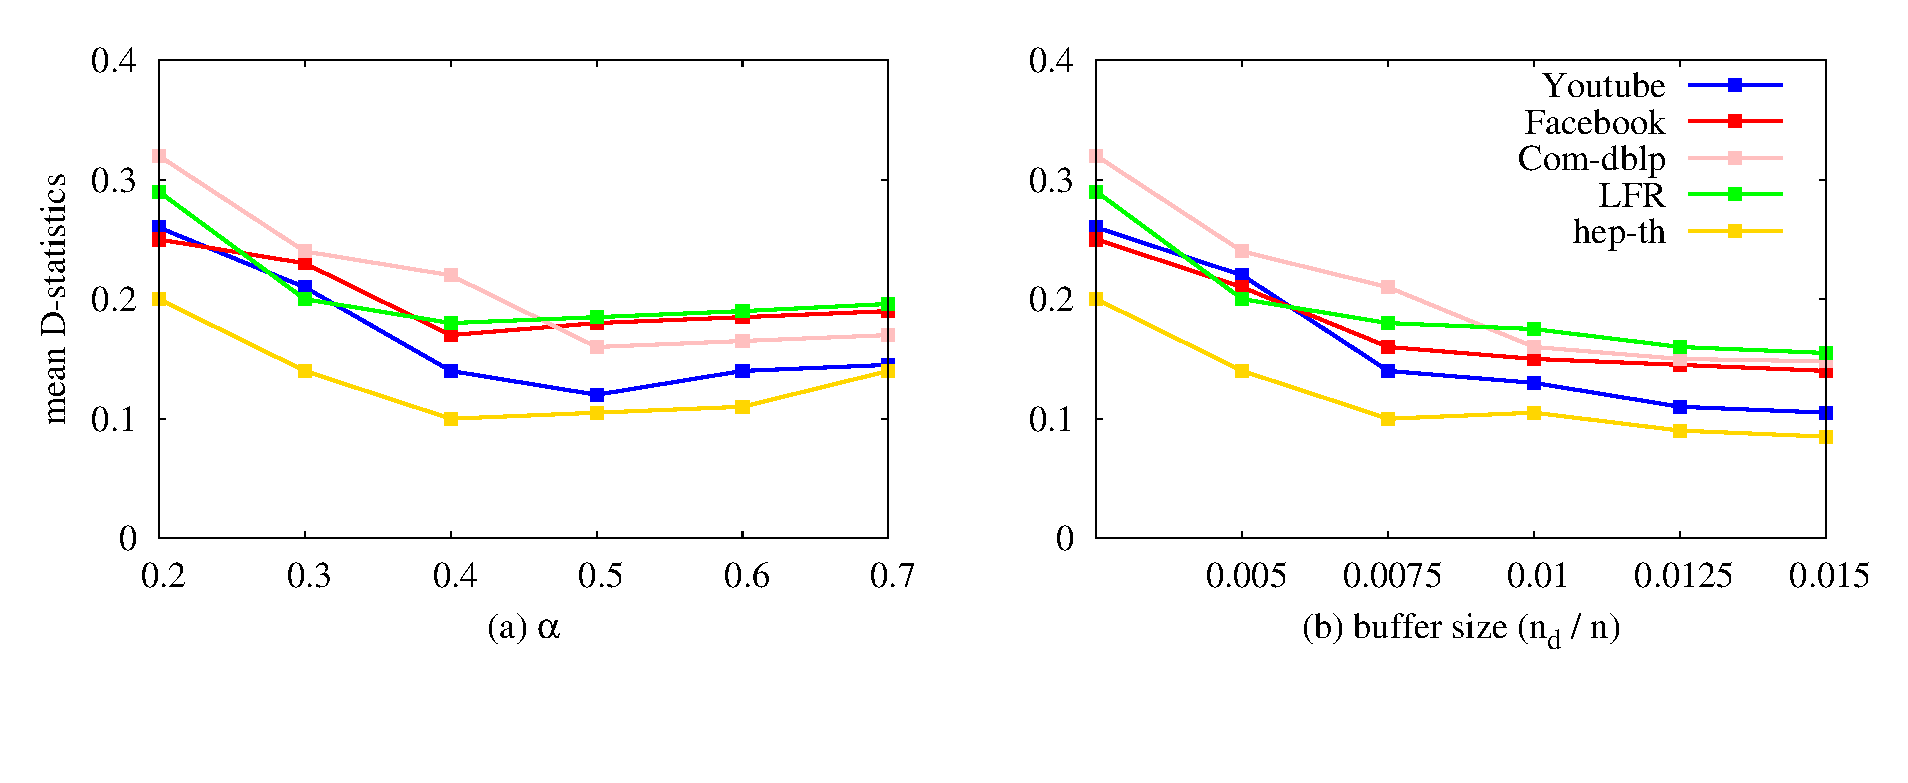
\includegraphics[width=0.8\columnwidth]{./texfiles/Chapter_2/figures/param_estimate.eps}
%\vspace{-12mm}
\caption{\label{param_est}Average $D$-statistics value across all the topological measures.}
\vspace{3mm}
%\vspace{-3mm}
\end{figure}


\iffalse
\begin{table}[!t]
\centering
\caption{\label{g_metric_alg}NMI between the ground-truth and community structure obtained from individual sampling algorithms for all datasets.}
%\scalebox{0.8}{
\begin{tabular}{l cccccc}
\hline
\multirow{1}{*}{{\bf Dataset}} & \multicolumn{1}{c}{{\bf \compas}} & \multicolumn{1}{c}{{\bf SN}} & \multicolumn{1}{c}{{\bf SE}} & \multicolumn{1}{c}{{\bf SBFS}} & \multicolumn{1}{c}{{\bf PIES}} & \multicolumn{1}{c}{{\bf GA}} \\\hline
Facebook	  & 0.52 & 0.34 & 0.28&0.41&0.48&0.61\\
hep-th		  &0.51&0.32&0.21&0.36&0.39&0.68\\
Youtube		      &0.72&0.49&0.33&0.58&0.51&0.77 \\
dblp		  &0.65&0.28&0.21&0.57&0.39&0.69 \\
LFR		  &0.69&0.29&0.32&0.38&0.31&0.72\\\hline
Average & {\bf 0.61}  & 0.34 & 0.27 & 0.46  & 0.41 & {\bf 0.69}    \\
\hline
\end{tabular}
%\vspace{4mm}
\end{table}
\fi
\begin{table}[!t]
\centering
\caption{\label{g_metric_alg}Purity (PU), NMI and ARI values between the ground-truth and community structure obtained from individual sampling algorithms for all datasets.}
\scalebox{0.68}{
\begin{tabular}{l |>{\columncolor[gray]{0.8}} c>{\columncolor[gray]{0.8}}  c>{\columncolor[gray]{0.8}}  c|  c  c  c| ccc|ccc|ccc|>{\columncolor[gray]{0.8}}c>{\columncolor[gray]{0.8}}c>{\columncolor[gray]{0.8}}c}
\hline
\multirow{2}{*}{{\bf Dataset}} & \multicolumn{3}{c|}{{\bf \compas}} & \multicolumn{3}{c|}{{\bf SN}} & \multicolumn{3}{c|}{{\bf SE}} & \multicolumn{3}{c|}{{\bf SBFS}} & \multicolumn{3}{c|}{{\bf PIES}} & \multicolumn{3}{c}{{\bf GA}} \\\cline{2-19}
   & \multicolumn{1}{c}{PU} & \multicolumn{1}{c}{NMI} & \multicolumn{1}{c|}{ARI} & PU & NMI & ARI &PU & NMI & ARI &PU & NMI & ARI &PU & NMI & ARI & \multicolumn{1}{c}{PU} & \multicolumn{1}{c}{NMI} & \multicolumn{1}{c}{ARI} \\\hline
Facebook	  & 0.71 & 0.52 & 0.47	 & 0.43&0.34&0.26  & 0.39&0.28&0.12  &  0.53&0.41&0.18  & 0.57&0.48&0.36  & 0.76&0.61&0.52 \\
hep-th		  &	0.69&0.51&0.38 & 0.39&0.32&0.19 & 0.29&0.21&0.12 & 0.42&0.36&0.25  & 0.48&0.39&0.31 & 0.74&0.68&0.57\\
youtube		      & 0.83&0.72&0.67	 &  0.52&0.49&0.36 & 0.48&0.33&0.28  &  0.63&0.58&0.47 & 0.56&0.51&0.41  & 0.86&0.77&0.71 \\
Dblp		  &	0.72&0.65&0.58 & 0.32&0.28&0.21  & 0.29&0.21&0.16  & 0.66&0.57&0.32  & 0.48&0.39&0.31  & 0.79&0.69&0.52 \\
LFR		  & 0.76&0.69&0.55	 & 0.35&0.29&0.21  & 0.56&0.32&0.29  & 0.49&0.38&0.26  & 0.42&0.31&0.28  &  0.81&0.72&0.67 \\\hline
Average & 0.74 & 0.61 & 0.53 & 0.40 & 0.34 & 0.24 & 0.40 & 0.27 &0.19 & 0.54 & 0.46 & 0.29 & 0.50 & 0.41 & 0.33 & 0.79 & 0.69 & 0.59   \\
\hline
\end{tabular}}
\vspace{3mm}
\end{table}


 {\bf Comparison of sampling algorithms}:
We start by measuring the similarity between the obtained and the ground-truth community structures using topological measures. In tables \ref{tab_fb},  \ref{tab_hep-th}, \ref{tab_yt}, \ref{tab_dblp} and \ref{tab_lfr} 
we summarize the $D$-statistics values of all the scoring functions for Facebook, arxiv hep-th, Youtube, dblp and LFR datasets respectively. 
%for the other graphs we only present the average value (and standard deviation) across the $D$-statistics for different topological 
%measures (detailed results on other datasets can be accessed in  \cite{si}). 
\iffalse\TODO{For these networks we MUST report standard deviation/error}.\fi 
Clearly~\compas~outperforms all the streaming algorithms across different datasets. GA performs better than~\compas~since it has in its 
consideration the whole graph to obtain the sample. However, we stress that even with {\em minimal community information to start with} and 
{\em no subsequent community detection in the later steps}, we are able to reach very close to GA as well as to the ground-truth.

Further we find \compas~is the second ranked algorithm after GA with an average 
(over all datasets) purity, NMI and ARI of {\bf 0.74}, {\bf 0.61} and {\bf 0.53} respectively (see table \ref{g_metric_alg} for detailed results). 
%(see Table \ref{g_metric_alg}  for NMI, details in \cite{si}).
\iffalse As a second level of evaluation, we further calculate three validation metrics -- purity, NMI and ARI  between the ground-truth and the obtained community structure for all the algorithms . Once again we observe that \\ \fi

\noindent{\bf Effect of edge ordering and sample size:}\label{sec:effect}
In this section, we show that most of our inferences are valid irrespective of any edge ordering. We randomly pick one pair of edges and swap their arrival time. 
We repeat it for $y$\% of edges (where $y$ varies between 5 and (as high as) 50) present in each aggregated graph. %\textcolor{red}{Put results starting from $x=5$ in steps of 5 up to 50.} 
%Each value of $x$ represents a new ordering with a higher value representing higher disorder. 
For each such ordering we obtain a representative sample (say $G_y$) and compare (average $D$-statistics)  with 
the ground-truth community. 
%the original graph ($S$). obtained considering the original arrival 
%order. The comparison is done by obtaining the distribution of each community scoring function for $S_x$ and $S$ and, subsequently, calculating the $D$-statistics.  
%For each value of $x$, we compare (through $D$-statistics) the distribution of each scoring function with the original order of edge arrivals. 
In figure~\ref{param_est_1}(a) we plot the $D$-statistics value averaged over all the scoring functions for the Youtube dataset. The plot clearly shows that the edge-ordering  
affects the final sample marginally.
%shows that for the Youtube graph edge ordering does not affect the final sample much (the pattern is same for LFR graph, see \cite{si}).
%\TODO{Mention how you obtained the ordering each time? Is it different random order or is there some strategic order also. You should make it explicit and say that~\compas~is tolerant to only these orders. DONE} 
%\textcolor{blue}{To obtain arrival sequences we consider two edges and swap their arrival times. This we do for 20\% of the total edges in the original network.

Lastly, we present the effect of sample size ($n$) on the obtained community structure. We plot average $D$-statistics values across all the topological measures for all the algorithms on Youtube as a function of $n$ (figure \ref{param_est_1}(b)). As expected, with the increase of $n$ we obtain better results. Interestingly, for~\compas~and GA, the pattern remains consistent compared to others. Moreover as we increase $n$ the divergence between their performance decreases.

%\vspace{-3mm}
\begin{figure}[!h]
\centering
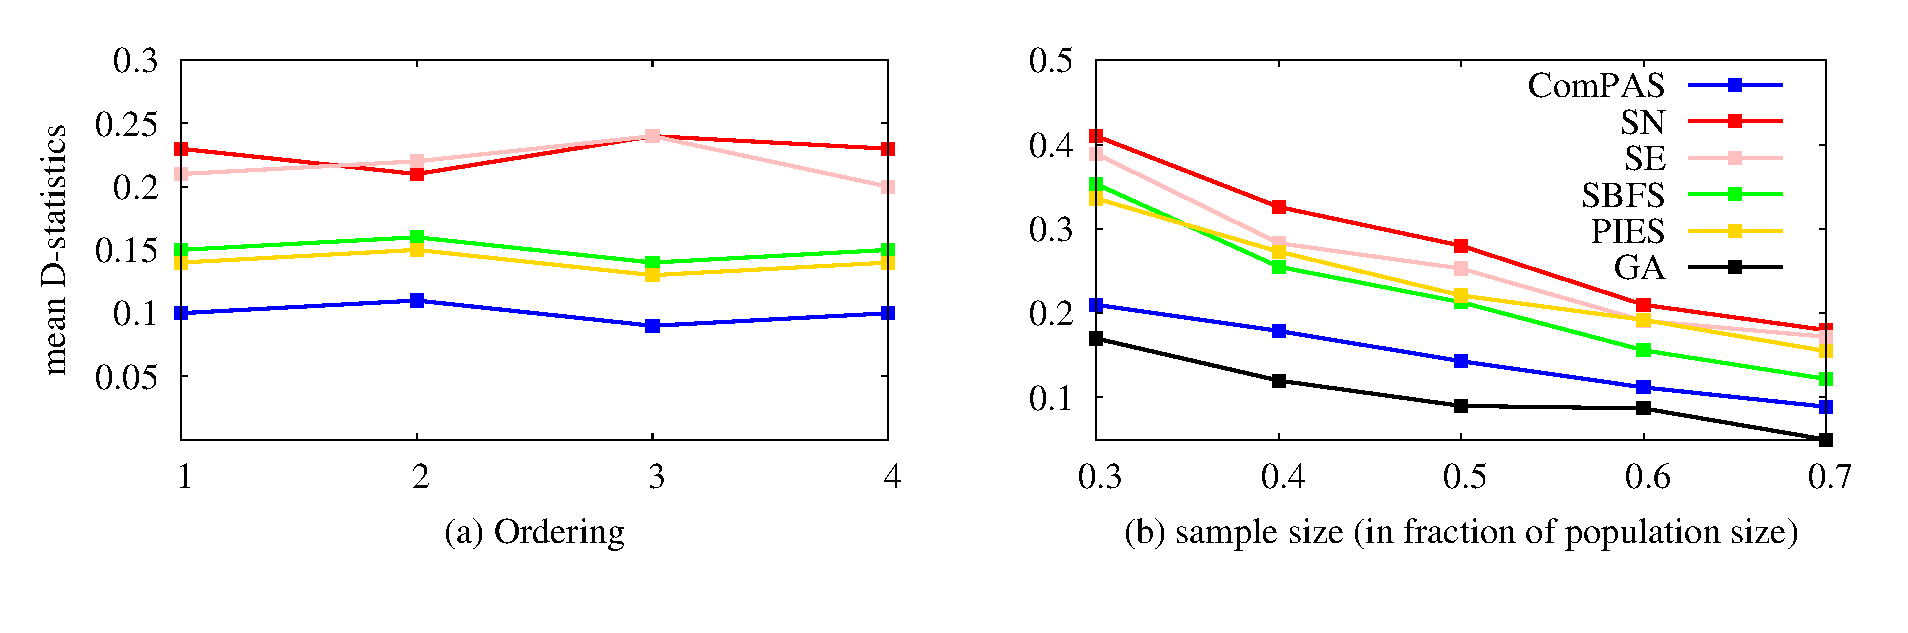
\includegraphics[width=0.8\columnwidth]{./texfiles/Chapter_2/figures/param_estimate_1.eps}
%\vspace{-10mm}
\caption{\label{param_est_1}Average $D$-statistics across all the topological measures for (a) different edge ordering and (b) sample size ($n$) of the Youtube graph.}
\vspace{4mm}
\end{figure}






%%%%%%%%%%%%%%%%%%%%%%%%%%%%%%%%%%%%%%%%%%%%%%%%%%%%%%%%%%%%%%%%%%%
\if{0}
{\bf Comment on edge-density of the sample}: 
Note that \compas~ is node-based, i.e., sample size is controlled by the number of nodes, and we at any point do not limit the number of edges in the sample ($e_{s}$). We compare the number of edges in the sample against that in the subgraph induced by the nodes in the obtained sample ($e_{p}$). 
We observe that on average our sample consists of only $\sim71$\% of the edges in the induced subgraph across all the datasets. 
%\iffalse\TODO{Sandipan: I had initially added a plot but decided against putting it as I felt it was not providing any extra information.}\fi
%which is followed by SBFS, PIES, SN and SE.
\iffalse
\subsection{Graph-centric evaluation}
\label{graph_evaluation}
We further evaluate our sample in terms of three graph properties mentioned in \cite{ahmed2014network}: (i) degree distribution (Degree), (ii) clustering coefficient distribution (CC), (iii) top 100 eigen value distribution (EV). 
Table \ref{graph_prop} reports the $D$-statistics values between the distributions of the original graph and those obtained from the sample (see more results in \cite{si}). For all the datasets, we observe that \compas~is within top three ranks in terms of low $D$-statistics, in many cases, also beating the strict baseline GA. This indicates that \compas~ also preserves general graphs properties in the sample.

\vspace{-2mm}
\begin{table}[!h]
\centering
\caption{Summary of $D$-statistics for different graph properties. For Youtube we present all the results, while for the rest we provide only average $D$-statistics (top three results in each average case are highlighted).}
\label{graph_prop}
\begin{adjustbox}{max width=\columnwidth}
\begin{tabular}{l|c c c |c|c|c|c|c}
\hline
  \multirow{2}{*}{Algorithm}         & \multicolumn{4}{c|}{Youtube}     & Facebook & Com-dblp & LFR     & hep-th  \\ \cline{2-9}
& Degree & CC & EV & Average & Average  & Average  & Average & Avearge \\ \hline
\compas    &   0.083     & 0.105   & 0.42     &  {\bf 0.20}       &  {\bf 0.17}        &  {\bf 0.16}       & {\bf 0.28}        & {\bf 0.18}       \\ 
SN        &    0.076    & 0.108   &  0.54     &  0.24             &   0.36             &  0.24             & 0.34              &  0.23       \\ 
SE        &    0.114    & 0.195   &  0.39     &  0.23             &   0.48             &  0.28             & 0.39              &  0.27       \\ 
SBFS      &    0.105    & 0.172   &  0.32     &  {\bf 0.19}       &   {\bf 0.28}       &  {\bf 0.13}       & {\bf 0.26}        & {\bf 0.19}       \\ 
PIES      &    0.046    &  0.129  &  0.38     &  {\bf 0.18}       &   {\bf 0.16}       &  0.21             & {\bf 0.28}        & {\bf 0.16}        \\ 
GA        &    0.218    &  0.063  &  0.46     &  0.24            &   0.35             &  {\bf 0.12}       & 0.32              &  0.20       \\ \hline
\end{tabular}
\end{adjustbox}
\vspace{-1mm}
\end{table}
\fi
%\vspace{-2mm} 

{\bf Effect of edge ordering and sample size:}
In this section, we show that most of our inferences are valid irrespective of any edge ordering. To do so, we randomly pick one pair of edges and swap their arrival time. 
We repeat it for $x$\% of edges (where $x$ varies between 5 and 50) present in each aggregated graph. %\textcolor{red}{Put results starting from $x=5$ in steps of 5 up to 50.} 
Each value of $x$ represents a new ordering with a higher 
value representing higher disorder. For each such ordering we obtain a representative sample (say $S_x$) and compare with sample ($S$) obtained considering original arrival 
order. The comparison is done by obtaining the distribution of each community scoring function for $S_x$ and $S$ and thereby calculating the $D$-statistics.  
%For each value of $x$, we compare (through $D$-statistics) the distribution of each scoring function with the original order of edge arrivals. 
In figure \ref{param_est_1}(a) we plot the $D$-statistics value averaged over all the scoring functions for Youtube dataset. 
The plot clearly shows that edge-ordering does not 
affect the final sample much. 
%(the pattern is same for LFR graph, see \cite{si}).
%\TODO{Mention how you obtained the ordering each time? Is it different random order or is there some strategic order also. You should make it explicit and say that~\compas~is tolerant to only these orders. DONE} 
%\textcolor{blue}{To obtain arrival sequences we consider two edges and swap their arrival times. This we do for 20\% of the total edges in the original network.
Lastly, we present the effect of sample size ($n$) on the obtained community structure. We plot average $D$-statistics values across all the topological measures for all the algorithms on Youtube  (see others in \cite{si}) as a function of $n$ (Figure \ref{param_est_1}(b)). As expected, with the increase of $n$ we obtain better results. Interestingly, for~\compas~and GA, the pattern remains consistent compared to others.\\


\noindent{\bf Extensions:} In its current form, our algorithm is applicable to undirected and and unweighted networks. We believe that through minor modifications our algorithm could be extended to 
directed as well as as weighted networks. \compas~ is aimed at optimizing modularity which has already been precisely defined for weighted~\cite{newman2004analysis} and 
directed networks~\cite{leicht2008community}. Further, the same sub-routines in the original algorithm, with minor modifications could be used for directed and weighted networks. 
The theoretical analysis would require additional research efforts which we plan to take up in future.

%\vspace{-5mm}
\begin{figure}[!h]
\centering
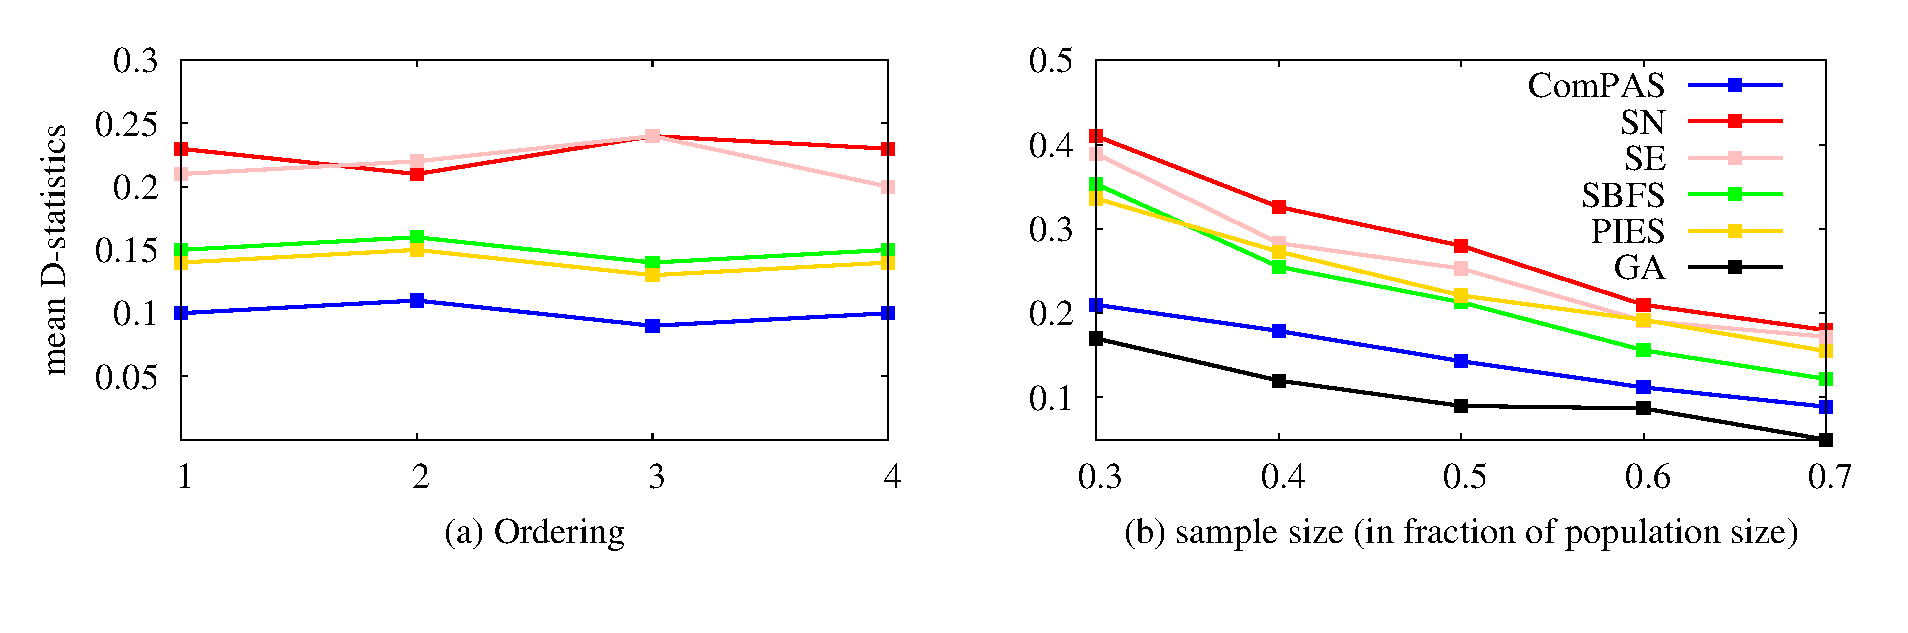
\includegraphics[width=0.8\columnwidth]{./texfiles/Chapter_2/figures/param_estimate_1.eps}
%\vspace{-10mm}
\caption{\label{param_est_1}Average $D$-statistics across all the topological measures for (a) different edge ordering and (b) sample size ($n$) of the Youtube graph.}
\vspace{4mm}
\end{figure}
\fi



%\if{0}

%\fi






%\section{Applications of compas}
Here we present two additional applications of \compas~-- ranking community detection algorithms, and selecting appropriate training set for (restricted) online learning. 
\subsection{Ranking community detection algorithms} As pointed out in \cite{maiya2010sampling}, there is always a trade-off between quality and running time for discovering the community structure from a graph. While some algorithms discover excellent community structure with larger running time, others compromise  quality by achieving lesser running time. Further, it is not possible to identify beforehand which community detection algorithm is more useful given a large graph. In this case, one is forced to run several algorithms on the large graph and converge on the best performing one. This may lead to a large computation cost and is especially detrimental in resource-scarce situations (absence of parallel infrastructures, distributed systems etc.).

In case of community detection on large streaming graphs, we 
posit that one may first execute \compas~and obtain a community-preserved sample. Then different community detection algorithms can be tested on the sample (which is much smaller in size compared to the original graph) and the best performing algorithm can be used for the original large graph. To this end, we execute five community detection (CD) algorithms (CNM \cite{clauset2004finding}, Fast-Greedy \cite{newman2004fast}, Walktrap \cite{pons2005computing}, Infomod \cite{rosvall2007information}, Infomop \cite{rosvall2008maps}) separately on each sample obtained from the sampling algorithms. Then we rank the CD algorithms based on their performance in terms of  modularity~\cite{newman2004analysis}. We further rank the CD algorithms in the same way considering the {\em entire graph}. We report the Kendall's $\tau$ rank correlation in Table~\ref{comp_wiki}(a) between these two ranks for individual sampling algorithms across all the datasets. We find GA and \compas~ performing the best. Therefore, \compas~can be used for selecting a CD algorithm quickly before running on a large streaming graph.

%This leads us to believe sample obtained through \compas~correctly ranks the performance of the community detection algorithms. 





\begin{table}[!t]
\centering
\caption{\label{comp_wiki} Rank correlation of community detection algorithms based on the performance on the sample (generated from individual sampling methods) and the original graph. (b) Performance of SVM using the training set obtained from sampling methods.}
\scalebox{0.71}{
\begin{tabular}{|c|c|c|c|c|c|c |c|c|}
\multicolumn{6}{c}{(a)} & \multicolumn{1}{c}{} & \multicolumn{2}{c}{(b)}\\ \cline{1-6}\cline{8-9}
Algo & Facebook & hep-th & Youtube & DBLP & LFR & &AUC & F-Score \\\cline{1-6}\cline{8-9}

\compas & {\bf 0.8} & {\bf 0.8} & {\bf 0.8} & {\bf 1.0} & {\bf 1.0}& & {\bf 0.48} & {\bf 0.61}  \\
SN & 0.4 & 0.6 & 0.4 &  0.6 & 0.6& & 0.31 & 0.35 \\
SE & 0.4 & 0.4& 0.4 &  0.6 & 0.4& & 0.25 & 0.28 \\
SBFS & 0.6 & 0.7 & 0.6 & 0.8 & 0.6& & 0.28 & 0.31 \\
PIES & 0.6 & 0.6 & 0.8 & 0.7 & 0.8& & 0.36 & 0.43\\
GA   & {\bf 1.0} & {\bf 0.8} & {\bf 0.8} & {\bf 1.0} & {\bf 1.0} & & {\bf 0.53} & {\bf 0.64} \\\cline{1-6}\cline{8-9}
\end{tabular}}
\end{table}


\subsection{Selecting training set for online learning}

In online learning, sometimes memory is limited and it is required to train the model on limited number of instances. In such situations it is important to choose a training set in such a way that it consists of members from most or all parts of the original dataset.

We hypothesize that more diverse the chosen set, better would be the performance. \compas~ is useful in such cases since it tries to sample from several communities, hence improving the diversity of the training set. To this end, we consider Wiki-Rfa\footnote{https://snap.stanford.edu/data/wiki-RfA.html} \cite{west2014exploiting}, a streaming signed graph in which nodes represent Wikipedia members and edges (with time-stamp) represent votes. Each vote is typically accompanied by a short comment. The task is to predict the vote (+1, 0, -1) of an incoming edge based on the textual features -- (i) word count, (ii) sentiment value, and (iii) LIWC features of the statement corresponding to the edge. We allow training instances to be included till a certain time period $t$ (first 75\% of the edges are allowed to enter) and run the sampling algorithms in parallel. However not all instances can be considered for training due to the memory constraint. We assume $n$, the sample size as the allowed training size and obtain sampled training set from individual sampling algorithms. We train SVM with linear kernel (see \cite{si} for other classifiers) on each sampled training set, and predict the labels (votes) of those instances coming after $t$. Table \ref{comp_wiki}(b) shows that GA and \compas~perform the best in terms of AUC and F-Score. 
 This once again emphasizes the fact that \compas~selects most representative training instances for (restricted) online learning.
 



\section{Summary of the chapter}
The contributions of this chapter can be summarized as follows - 
\begin{itemize}
 \item We proposed \compas, a novel sampling algorithm for streaming graphs 
which is able to retain the community structure of the original graph.
 \item Through rigorous experimentation on four real-world and one synthetic graphs we showed that our algorithm performs better than 
five state-of-the-art graph sampling algorithms.
 \item We further showed the effectiveness of \compas~ in online learning frameworks
\end{itemize}
  
A possible future direction would be to analytically estimate the relation between sample size and the accuracy of our algorithm. 
It would also be interesting to investigate in detail the effectiveness of \compas~ in other real applications. 

%We also plan to check whether the present algorithm could be modified to estimate multiple graph properties. Finally we plan to extend our work to directed and weighted networks.  


%\appendix
%PROPOSITION 1.
{\em
For a community $c\in C$, if $D_c\leq M-1$ then addition of an edge within $c$ will increase its modularity.}

\begin{proof}
From Equation \ref{modularity}, we see the contribution of individual community $c\in C$ in modularity as: $Q_c=\frac{m_c}{M} - \frac{D_c^2}{4M^2}$. 
where $m_c$ is the number of edges inside $c$, $M$ is the total number of edges in the graph, and $D_c$ is the sum of degrees of all the nodes in $c$. 

Addition of a new edge within $c$, the $c$'s contribution of modularity becomes:
\[
Q'_c=\frac{m_c+1}{M+1} - \frac{(D_c+2)^2}{4(M+1)^2}
\]

So the increase in modularity is $\Delta Q_c=Q'_c-Q_c$,
\[\small
\begin{split}
\Delta Q_c=&\frac{4M^2-4m_cM^2-4D_cM^2-4m_cM+2D_c^2M+D_c^2}{4(M+1)^2M^2}\\
&\geq \frac{4M^2-6D_cM^2-2D_cM+2D_c^2M+D_c^2}{4(M+1)^2M^2}\\
&\geq\frac{(2M^2-2D_cM-D_c)(2M-D_c)}{4(M+1)^2M^2}\\
&\geq 0
\end{split}
\]
The equality holds if $D_c\leq M-1$. This thus implies $(2M^2-2D_cM-D_c)\geq 0$. This proves the proposition.
\end{proof}

PROPOSITION 2.
{\em For a community $c\in C$, addition of any intra-community edge into $c$ should not split it into smaller communities.}


\begin{proof}
We will prove this proposition by contradiction.
Assume that once a new intra-community edge is added into $c$, it gets split into $k$ small modules, namely $X_1$, $X_2$, $\cdot$,$X_k$. Let $D_{X_i}$ and $e_{ij}$ be the total degree of nodes inside $X_i$ and number of edges connecting $X_i$ and $X_j$ respectively. 


Recall that the contribution of $X_i$ in the modularity value is $Q_{X_i}=\frac{m_{X_i}}{M} - \frac{D_{X_i}^2}{4M^2}$.  Before adding the edge, we have $Q_c \geq \sum_{i=1}^k Q_{X_i}$ (where $Q_c$ is the total modularity of community $c$), because otherwise all $X_i$s can be split earlier, which is not in this case. This implies that:
\[
\frac{m_c}{M}- \frac{D_c^2}{4M^2} > \sum_{i=1}^k (\frac{m_{X_i}}{M} - \frac{D_{X_i}^2}{4M^2})
\]
Since $X_1,X_2,\cdot,X_k$ are all disjoint modules of $c$, $D_c=\sum_{i=1}^k D_{X_i}$ and $m_c=\sum_{i=1}^k m_{X_i} + \sum_{i<j} e_{ij}$. This further implies that:
\[
\frac{m_c}{M}-\sum_{i=1}^k \frac{m_{X_i}}{M} > \frac{D_c^2}{4M^2}- \sum_{i=1}^k \frac{D_{X_i}^2}{4M^2}
\]
or,
\[
\sum_{i<j} e_{ij} > \frac{\sum_{i<j} D_{X_i}D_{X_j}}{2M}
\]
 
 Without loss of generality, let us assume that the new edge is added inside $X_1$. 
Since we assume that after adding the new edge into $c$, it gets split into $k$ small modules, the modularity value should increase because of the split. Therefore, the new modularity $Q'_c<\sum_{i=1}^k Q_{X_i}$. This implies that
\[\small
\begin{split}\small
& Q'_c < \sum_{i=1}^k Q_{X_i}\\
& \Leftrightarrow \frac{\sum_{i=1}^k m_{X_i} + \sum_{i<j} e_{ij} + 1}{M+1} - \frac{(\sum_{i=1}^k D_{X_i +2})^2}{4(M+1)^2}\\
& <  \frac{m_{X_1}+1}{M+1} - \frac{(D_{X_1}+2)^2}{4(M+1)^2}  + \sum_{i=2}^k  (\frac{m_{X_i}}{M+1} - \frac{D_{X_i}^2}{4(M+1)^2} )\\
&\Leftrightarrow \frac{\sum_{i=1}^k m_{X_i} + \sum_{i<j} e_{ij} + 1}{M+1} - \frac{(\sum_{i=1}^k D_{X_i +2})^2}{4(M+1)^2}\\
& < \frac{\sum_{i=1}^k m_{X_i}+1}{M+1} - \frac{(D_{X_1}+2)^2}{4(M+1)^2} - \sum_{i=2}^k \frac{D_{X_i}^2}{4(M+1)^2}\\
&\Leftrightarrow \sum_{i<i} e_{ij} < \frac{\sum_{i=1}^k D_{X_i} - 2 D_{X_1} + \sum_{i<j} D_{X_i}D_{X_j}}{2(M+1)}
\end{split}
\]
Since $\sum_{i=1}^k D_{X_i} - 2D_{X_1} < 2M$, this implies that 
\[\small
\begin{split}
\frac{\sum_{i<j}D_{X_i}D_{X_j}}{2M}  < \sum_{i<j}e_{ij} 
&< \frac{\sum_{i=1}^k D_{X_i} - 2D_{X_1} + \sum_{i\neq j}{D_{X_i}D_{X_j}}}{2(M+1)}\\
& <\frac{\sum_{i<j}D_{X_i}D_{X_j}}{2M}+1
\end{split}
\]
Therefore, the proposition holds.
\end{proof}





PROPOSITION 3.
{\em If a new edge $(u,v)$ connecting two communities $C(u)$ and $C(v)$ is introduced, $C(u)$ $($or $C(v))$ is the best candidate for $v$ (or $u$) if it should ever change its community membership.}

\begin{proof}
The method is inspired by \cite{PhysRevE.78.046115} that a vertex $u$ is influenced by two factors: $F^c_{in}(u)$ the force that keeps $u$ stay in its own community $c$, and $F^c_{out}(u)$, the force that a community $S$ imposes to $u$ in order to bring $u$ to $S$ as follows:
\[
F^c_{in}(u)=e_c^u-\frac{d_u(D_c-d_u)}{2M}
\]
and 
\[
F^S_{out}(u)=max_{S\in NC(u)} \{e_S^u - \frac{d_u D_{outS}}{2M}\}
\]
where $NC(u)$ is the set of neighboring communities of $u$, and $D_{outS}$ is the total degree of vertices outside $S$.

Now we will show that the presence of new edge $(u,v)$ will strengthen $F^{C(v)}_{out}(u)$ and weaken $F^S_{out}(u)$. In other words, we will show that $F^{C(v)}_{out}(u)$ increases while $F^S_{out}(u)$ decreases for all $S \in C \wedge S \notin \{C(u),C(v)\}$.
\[\small
\begin{split}
&F^{C(v)}_{out}(u)|_{new} - F^{C(v)}_{out}(u)|_{old}\\
&=(e_u^{C(v)}+1-\frac{(d_u+1)(d_{outC(v)}+1)}{2(M+1)} - (e_u^{C(v)} - \frac{d_ud_{outC(v)}}{2M})\\
&= \frac{2M+d_ud_{outC(v)}}{2(M+1)} - \frac{d_ud_{outC(v)}+d_{outD(v)}+d_u+1}{2(M+1)}\\
&\geq \frac{2M+d_ud_{outC(v)}}{2(M+1)} - \frac{d_u d_{outC(v)}+d_{outC(v)}+d_u+1}{2(M+1)}\\
&>0
\end{split}
\]
Therefore $F^{C(v)}_{out}(u)$ is strengthen when new edge $(u,v)$ is introduced. Furthermore, for any community $S\in C \wedge S\notin \{C(u),C(v)\}$
\[
\begin{split}
& F^{S}_{out}(u)|_{new} - F^{S}_{out}(u)|_{old}\\
&= (e^S_u-\frac{(d_u+1)d_{outS}}{2(M+1)}) - (e^S_u - \frac{d_ud_{outS}}{2M})\\
&= d_{outS}(\frac{d_u}{2M} - \frac{d_u+1}{2(M+1)})<0
\end{split}
\]

This implies that $F^S_{out}(u)$ is weakened when $(u,v)$ is added. Therefore,  the proposition holds.
\end{proof}


PROPOSITION 4.
{\em If a new edge $(u,v)$ is added into the network, then joining $u$ to $v$'s $C(v)$ community will increase the modularity value  if $\Delta Q(u,C(u),C(v)) \equiv 4(M+1)(e_{C(v)}^u+1-e_{C(u)}^u)+e_{C(v)}^u(2D_{C(v)}-2d_u-e_{C(u)}^u) - 2(d_u+1)(d_u+1+d_{C(v)}-d_{C(u)})>0$.}

\begin{proof}
Vertex $u$ will leave its current community $C(u)$ and join $v$'s community $C(v)$ if\\
\[\scriptsize
\begin{split}
& Q_{C(v)+u} + Q_{C(u)-u} > Q_{c(u)} + Q_{C(v)}\\
&\Leftrightarrow \frac{m_{C(v)}+e_{C(v)}+1}{M+1} - \frac{(d_{C(v)}+d_u+2)^2}{4(M+1)^2}+\\
&\frac{m_{C(u)} - e_{C(u)}}{M+1} - \frac{(d_{C(u)}-d_u-e_{C(u)})}{4(M+1)^2} \\
& > \frac{m_{C(v)}}{M+1} - \frac{(d_{C(v)}+d_u+2)^2}{4(M+1)^2} + \frac{m_{C(u)}}{M+1} - \frac{(d_{C(u)}+1)^2}{4(M+1)^2}\\
&\Leftrightarrow 4(M+1)(e_{C(v)} +1 -e_{C(u)}) + e_{C(u)}(2d_{C(v)} - 2d_{C(u)}-e_{C(u)})\\
& - 2(d_{C(u)}+1)(d_{C(u)}+1+d_{C(v)}-d_{C(u)})>0
\end{split}\]
\end{proof}


\newpage
%\bibliographystyle{abbrv}
%\bibliography{sigproc} 
%\end{document}


